\documentclass[twoside]{book}

% Packages required by doxygen
\usepackage{fixltx2e}
\usepackage{calc}
\usepackage{doxygen}
\usepackage[export]{adjustbox} % also loads graphicx
\usepackage{graphicx}
\usepackage[utf8]{inputenc}
\usepackage{makeidx}
\usepackage{multicol}
\usepackage{multirow}
\PassOptionsToPackage{warn}{textcomp}
\usepackage{textcomp}
\usepackage[nointegrals]{wasysym}
\usepackage[table]{xcolor}

% Font selection
\usepackage[T1]{fontenc}
\usepackage[scaled=.90]{helvet}
\usepackage{courier}
\usepackage{amssymb}
\usepackage{sectsty}
\renewcommand{\familydefault}{\sfdefault}
\allsectionsfont{%
  \fontseries{bc}\selectfont%
  \color{darkgray}%
}
\renewcommand{\DoxyLabelFont}{%
  \fontseries{bc}\selectfont%
  \color{darkgray}%
}
\newcommand{\+}{\discretionary{\mbox{\scriptsize$\hookleftarrow$}}{}{}}

% Page & text layout
\usepackage{geometry}
\geometry{%
  a4paper,%
  top=2.5cm,%
  bottom=2.5cm,%
  left=2.5cm,%
  right=2.5cm%
}
\tolerance=750
\hfuzz=15pt
\hbadness=750
\setlength{\emergencystretch}{15pt}
\setlength{\parindent}{0cm}
\setlength{\parskip}{0.2cm}
\makeatletter
\renewcommand{\paragraph}{%
  \@startsection{paragraph}{4}{0ex}{-1.0ex}{1.0ex}{%
    \normalfont\normalsize\bfseries\SS@parafont%
  }%
}
\renewcommand{\subparagraph}{%
  \@startsection{subparagraph}{5}{0ex}{-1.0ex}{1.0ex}{%
    \normalfont\normalsize\bfseries\SS@subparafont%
  }%
}
\makeatother

% Headers & footers
\usepackage{fancyhdr}
\pagestyle{fancyplain}
\fancyhead[LE]{\fancyplain{}{\bfseries\thepage}}
\fancyhead[CE]{\fancyplain{}{}}
\fancyhead[RE]{\fancyplain{}{\bfseries\leftmark}}
\fancyhead[LO]{\fancyplain{}{\bfseries\rightmark}}
\fancyhead[CO]{\fancyplain{}{}}
\fancyhead[RO]{\fancyplain{}{\bfseries\thepage}}
\fancyfoot[LE]{\fancyplain{}{}}
\fancyfoot[CE]{\fancyplain{}{}}
\fancyfoot[RE]{\fancyplain{}{\bfseries\scriptsize Generated on Mon Mar 9 2015 21\+:04\+:06 for Delta\+Robot by Doxygen }}
\fancyfoot[LO]{\fancyplain{}{\bfseries\scriptsize Generated on Mon Mar 9 2015 21\+:04\+:06 for Delta\+Robot by Doxygen }}
\fancyfoot[CO]{\fancyplain{}{}}
\fancyfoot[RO]{\fancyplain{}{}}
\renewcommand{\footrulewidth}{0.4pt}
\renewcommand{\chaptermark}[1]{%
  \markboth{#1}{}%
}
\renewcommand{\sectionmark}[1]{%
  \markright{\thesection\ #1}%
}

% Indices & bibliography
\usepackage{natbib}
\usepackage[titles]{tocloft}
\setcounter{tocdepth}{3}
\setcounter{secnumdepth}{5}
\makeindex

% Hyperlinks (required, but should be loaded last)
\usepackage{ifpdf}
\ifpdf
  \usepackage[pdftex,pagebackref=true]{hyperref}
\else
  \usepackage[ps2pdf,pagebackref=true]{hyperref}
\fi
\hypersetup{%
  colorlinks=true,%
  linkcolor=blue,%
  citecolor=blue,%
  unicode%
}

% Custom commands
\newcommand{\clearemptydoublepage}{%
  \newpage{\pagestyle{empty}\cleardoublepage}%
}


%===== C O N T E N T S =====

\begin{document}

% Titlepage & ToC
\hypersetup{pageanchor=false,
             bookmarks=true,
             bookmarksnumbered=true,
             pdfencoding=unicode
            }
\pagenumbering{roman}
\begin{titlepage}
\vspace*{7cm}
\begin{center}%
{\Large Delta\+Robot \\[1ex]\large v0.\+1 }\\
\vspace*{1cm}
{\large Generated by Doxygen 1.8.9.1}\\
\vspace*{0.5cm}
{\small Mon Mar 9 2015 21:04:06}\\
\end{center}
\end{titlepage}
\clearemptydoublepage
\tableofcontents
\clearemptydoublepage
\pagenumbering{arabic}
\hypersetup{pageanchor=true}

%--- Begin generated contents ---
\chapter{Hierarchical Index}
\section{Class Hierarchy}
This inheritance list is sorted roughly, but not completely, alphabetically\+:\begin{DoxyCompactList}
\item \contentsline{section}{data}{\pageref{structdata}}{}
\item \contentsline{section}{dxl\+\_\+hal}{\pageref{classdxl__hal}}{}
\item \contentsline{section}{dynamixel}{\pageref{classdynamixel}}{}
\item \contentsline{section}{dynamixel2}{\pageref{classdynamixel2}}{}
\item \contentsline{section}{X\+Joystick\+:\+:Info}{\pageref{struct_x_joystick_1_1_info}}{}
\item \contentsline{section}{ping\+\_\+data}{\pageref{structping__data}}{}
\item Q\+Dialog\begin{DoxyCompactList}
\item \contentsline{section}{Options\+Window}{\pageref{class_options_window}}{}
\end{DoxyCompactList}
\item Q\+Main\+Window\begin{DoxyCompactList}
\item \contentsline{section}{Main\+Window}{\pageref{class_main_window}}{}
\end{DoxyCompactList}
\item Q\+Object\begin{DoxyCompactList}
\item \contentsline{section}{A\+X12}{\pageref{class_a_x12}}{}
\item \contentsline{section}{X\+Joystick}{\pageref{class_x_joystick}}{}
\end{DoxyCompactList}
\item Q\+Widget\begin{DoxyCompactList}
\item \contentsline{section}{Options\+Servos}{\pageref{class_options_servos}}{}
\end{DoxyCompactList}
\end{DoxyCompactList}

\chapter{Class Index}
\section{Class List}
Here are the classes, structs, unions and interfaces with brief descriptions\+:\begin{DoxyCompactList}
\item\contentsline{section}{\hyperlink{class_a_x12}{A\+X12} \\*Used to control A\+X-\/12 motors from Dynamixel }{\pageref{d1/daa/class_a_x12}}{}
\item\contentsline{section}{\hyperlink{struct_x_joystick_1_1_axis}{X\+Joystick\+::\+Axis} \\*Struct to handle the axis }{\pageref{d2/d0a/struct_x_joystick_1_1_axis}}{}
\item\contentsline{section}{\hyperlink{structdata}{data} }{\pageref{df/dea/structdata}}{}
\item\contentsline{section}{\hyperlink{classdxl__hal}{dxl\+\_\+hal} }{\pageref{d5/dae/classdxl__hal}}{}
\item\contentsline{section}{\hyperlink{classdynamixel}{dynamixel} }{\pageref{df/d7e/classdynamixel}}{}
\item\contentsline{section}{\hyperlink{classdynamixel2}{dynamixel2} }{\pageref{d9/deb/classdynamixel2}}{}
\item\contentsline{section}{\hyperlink{struct_x_joystick_1_1_info}{X\+Joystick\+::\+Info} \\*Struct to handle the info }{\pageref{dd/de5/struct_x_joystick_1_1_info}}{}
\item\contentsline{section}{\hyperlink{class_main_window}{Main\+Window} }{\pageref{d9/dc6/class_main_window}}{}
\item\contentsline{section}{\hyperlink{class_options_servos}{Options\+Servos} }{\pageref{da/dec/class_options_servos}}{}
\item\contentsline{section}{\hyperlink{class_options_window}{Options\+Window} }{\pageref{d7/d60/class_options_window}}{}
\item\contentsline{section}{\hyperlink{structping__data}{ping\+\_\+data} }{\pageref{d5/dab/structping__data}}{}
\item\contentsline{section}{\hyperlink{class_x_joystick}{X\+Joystick} \\*The \hyperlink{class_x_joystick}{X\+Joystick}\textquotesingle{}s class is used to control the S\+F\+M\+L Joystick\textquotesingle{}s class with {\itshape signals and slots} }{\pageref{dc/dc5/class_x_joystick}}{}
\end{DoxyCompactList}

\chapter{Class Documentation}
\hypertarget{class_a_x12}{}\section{A\+X12 Class Reference}
\label{class_a_x12}\index{A\+X12@{A\+X12}}


The \hyperlink{class_a_x12}{A\+X12} class is used to control A\+X-\/12 motors from Dynamixel.  




{\ttfamily \#include $<$ax12.\+h$>$}



Inheritance diagram for A\+X12\+:

\hypertarget{structdata}{}\section{data Struct Reference}
\label{structdata}\index{data@{data}}


{\ttfamily \#include $<$dynamixel.\+h$>$}

\subsection*{Public Attributes}
\begin{DoxyCompactItemize}
\item 
unsigned char \hyperlink{structdata_a5a553f5c59b2c973d161ea3352c32d07}{i\+I\+D}
\item 
unsigned int \hyperlink{structdata_a849125c9807b08e525118cdca5a255fe}{i\+Start\+Addr}
\item 
unsigned short \hyperlink{structdata_a836daaa4328239851986211241acbcca}{i\+Length}
\item 
unsigned char \hyperlink{structdata_a907d6311fb7b92b5960df0bef3b32c43}{i\+Error}
\item 
unsigned char $\ast$ \hyperlink{structdata_a03c940df871cecb40e4f5ca39f14cc49}{puc\+Table}
\end{DoxyCompactItemize}


\subsection{Member Data Documentation}
\hypertarget{structdata_a907d6311fb7b92b5960df0bef3b32c43}{}\index{data@{data}!i\+Error@{i\+Error}}
\index{i\+Error@{i\+Error}!data@{data}}
\subsubsection[{i\+Error}]{\setlength{\rightskip}{0pt plus 5cm}unsigned char data\+::i\+Error}\label{structdata_a907d6311fb7b92b5960df0bef3b32c43}
\hypertarget{structdata_a5a553f5c59b2c973d161ea3352c32d07}{}\index{data@{data}!i\+I\+D@{i\+I\+D}}
\index{i\+I\+D@{i\+I\+D}!data@{data}}
\subsubsection[{i\+I\+D}]{\setlength{\rightskip}{0pt plus 5cm}unsigned char data\+::i\+I\+D}\label{structdata_a5a553f5c59b2c973d161ea3352c32d07}
\hypertarget{structdata_a836daaa4328239851986211241acbcca}{}\index{data@{data}!i\+Length@{i\+Length}}
\index{i\+Length@{i\+Length}!data@{data}}
\subsubsection[{i\+Length}]{\setlength{\rightskip}{0pt plus 5cm}unsigned short data\+::i\+Length}\label{structdata_a836daaa4328239851986211241acbcca}
\hypertarget{structdata_a849125c9807b08e525118cdca5a255fe}{}\index{data@{data}!i\+Start\+Addr@{i\+Start\+Addr}}
\index{i\+Start\+Addr@{i\+Start\+Addr}!data@{data}}
\subsubsection[{i\+Start\+Addr}]{\setlength{\rightskip}{0pt plus 5cm}unsigned int data\+::i\+Start\+Addr}\label{structdata_a849125c9807b08e525118cdca5a255fe}
\hypertarget{structdata_a03c940df871cecb40e4f5ca39f14cc49}{}\index{data@{data}!puc\+Table@{puc\+Table}}
\index{puc\+Table@{puc\+Table}!data@{data}}
\subsubsection[{puc\+Table}]{\setlength{\rightskip}{0pt plus 5cm}unsigned char$\ast$ data\+::puc\+Table}\label{structdata_a03c940df871cecb40e4f5ca39f14cc49}


The documentation for this struct was generated from the following file\+:\begin{DoxyCompactItemize}
\item 
\hyperlink{dynamixel_8h}{dynamixel.\+h}\end{DoxyCompactItemize}

\hypertarget{classdxl__hal}{}\section{dxl\+\_\+hal Class Reference}
\label{classdxl__hal}\index{dxl\+\_\+hal@{dxl\+\_\+hal}}
\subsection*{Public Member Functions}
\begin{DoxyCompactItemize}
\item 
\hypertarget{classdxl__hal_a5b91f0f0b4a61fa113f9919e07e5a329}{}int {\bfseries open} (Q\+String \&dev\+Name, int baudrate)\label{classdxl__hal_a5b91f0f0b4a61fa113f9919e07e5a329}

\item 
\hypertarget{classdxl__hal_a250fd7e4acabf54d0733551a13e89a2d}{}void {\bfseries close} (void)\label{classdxl__hal_a250fd7e4acabf54d0733551a13e89a2d}

\item 
\hypertarget{classdxl__hal_a004eedde5af69219d7288ec8ea97c89f}{}void {\bfseries clear} (void)\label{classdxl__hal_a004eedde5af69219d7288ec8ea97c89f}

\item 
\hypertarget{classdxl__hal_a0eaaa5340bc9dce73cc920dc8befe5b0}{}int {\bfseries change\+\_\+baudrate} (float baudrate)\label{classdxl__hal_a0eaaa5340bc9dce73cc920dc8befe5b0}

\item 
\hypertarget{classdxl__hal_a90106970438fb0ab65852730a1c0776a}{}int {\bfseries write} (unsigned char $\ast$p\+Packet, int num\+Packet)\label{classdxl__hal_a90106970438fb0ab65852730a1c0776a}

\item 
\hypertarget{classdxl__hal_ac36331febb2eaa66303af3483795742a}{}int {\bfseries read} (unsigned char $\ast$p\+Packet, int num\+Packet)\label{classdxl__hal_ac36331febb2eaa66303af3483795742a}

\item 
\hypertarget{classdxl__hal_a6b6b7381c45308662fc3df6e7f74bc61}{}double {\bfseries get\+\_\+curr\+\_\+time} ()\label{classdxl__hal_a6b6b7381c45308662fc3df6e7f74bc61}

\item 
\hypertarget{classdxl__hal_a88bba601b5c9f285fcdc14e18a1f3398}{}bool {\bfseries is\+Open} ()\label{classdxl__hal_a88bba601b5c9f285fcdc14e18a1f3398}

\end{DoxyCompactItemize}


The documentation for this class was generated from the following files\+:\begin{DoxyCompactItemize}
\item 
dxl\+\_\+hal.\+h\item 
dxl\+\_\+hal.\+cpp\end{DoxyCompactItemize}

\hypertarget{classdynamixel}{}\section{dynamixel Class Reference}
\label{classdynamixel}\index{dynamixel@{dynamixel}}


Dynamixel 1.\+0 protocol class.  




{\ttfamily \#include $<$dynamixel.\+h$>$}



Collaboration diagram for dynamixel\+:\nopagebreak
\begin{figure}[H]
\begin{center}
\leavevmode
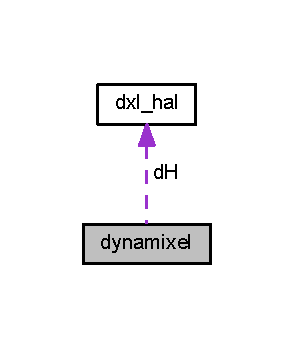
\includegraphics[width=141pt]{df/d4c/classdynamixel__coll__graph}
\end{center}
\end{figure}
\subsection*{Public Member Functions}
\begin{DoxyCompactItemize}
\item 
\hyperlink{classdynamixel_a7aa668a213db6a41bede8e08a6fec830}{dynamixel} ()
\item 
\hyperlink{classdynamixel_a5d4fed957a4b2d1690c0fa72127f5cbf}{dynamixel} (Q\+String port\+\_\+num, int baud\+\_\+rate=1000000)
\item 
bool \hyperlink{classdynamixel_a5ae4b2c6eb4c91f404f973ee8e6a1914}{is\+Open} ()
\item 
int \hyperlink{classdynamixel_a87960244d5846ae7583e37d2407eb61e}{initialize} (Q\+String port\+\_\+num, int baud\+\_\+rate)
\item 
int \hyperlink{classdynamixel_a7554c7889896e29e11a62027d89f3fdf}{change\+\_\+baudrate} (int baud\+\_\+rate)
\item 
int \hyperlink{classdynamixel_a92ea074ed1c1a9cf29e039f8c425f01a}{terminate} (void)
\item 
int \hyperlink{classdynamixel_ac8440d5d34ae3c4618b28fdbbd748edc}{get\+\_\+comm\+\_\+result} ()
\item 
void \hyperlink{classdynamixel_a479187cd8940c16dd4374eb5be22b888}{tx\+\_\+packet} (void)
\item 
void \hyperlink{classdynamixel_aa26d2d2dff768563a1cb1480aa061608}{rx\+\_\+packet} (void)
\item 
void \hyperlink{classdynamixel_aebfc569c6b1eb0b98f8c385f0f921fc0}{txrx\+\_\+packet} (void)
\item 
void \hyperlink{classdynamixel_a84e24c72c3e5be866f8b28c2e5bd1d95}{set\+\_\+txpacket\+\_\+id} (int id)
\item 
void \hyperlink{classdynamixel_a209a43f983f214323b6f0a627d5e8c13}{set\+\_\+txpacket\+\_\+instruction} (int instruction)
\item 
void \hyperlink{classdynamixel_a2c3d31bbbed70a69918e9972a620384b}{set\+\_\+txpacket\+\_\+parameter} (int index, int value)
\item 
void \hyperlink{classdynamixel_a829278f48e21c810b172eb8cab3b86de}{set\+\_\+txpacket\+\_\+length} (int length)
\item 
int \hyperlink{classdynamixel_a1bbabb82d7a2764cc4b0b351dd0019e5}{get\+\_\+rxpacket\+\_\+error} (int error)
\item 
int \hyperlink{classdynamixel_a6e62341ef9f51b6e152e769bd7be9d75}{get\+\_\+rxpacket\+\_\+error\+\_\+byte} (void)
\item 
int \hyperlink{classdynamixel_a68b5fa99719a9aec0734ecfb0635503b}{get\+\_\+rxpacket\+\_\+parameter} (int index)
\item 
int \hyperlink{classdynamixel_ae9cc18fdeda8329f68fa0f2f0a7a9aba}{get\+\_\+rxpacket\+\_\+length} ()
\item 
void \hyperlink{classdynamixel_af2bd714423e7c4fc089762805c0c71f3}{ping} (int id)
\item 
int \hyperlink{classdynamixel_a888404b41c4c4395a0b745c77ff2cea9}{read\+\_\+byte} (int id, int address)
\item 
void \hyperlink{classdynamixel_a66c1e32cc45dd46d329f1fc212e46a3d}{write\+\_\+byte} (int id, int address, int value)
\item 
int \hyperlink{classdynamixel_a45e99341e82c5114f6e829c9141bf96f}{read\+\_\+word} (int id, int address)
\item 
void \hyperlink{classdynamixel_a925f62ce5e261e5ef4fe6dc46bdc7c63}{write\+\_\+word} (int id, int address, int value)
\item 
double \hyperlink{classdynamixel_a2fa5375537184c279a9ebfcfc0425071}{get\+\_\+packet\+\_\+time} ()
\item 
void \hyperlink{classdynamixel_a067f82c21ed176e18fa224d16f3d1c5b}{set\+\_\+packet\+\_\+timeout} (int Num\+Rcv\+Byte)
\item 
void \hyperlink{classdynamixel_a125b42f776c4aac520f274074f68b591}{set\+\_\+packet\+\_\+timeout\+\_\+ms} (int msec)
\item 
int \hyperlink{classdynamixel_afddd976dbc486cd08b92e0e6e4117519}{is\+\_\+packet\+\_\+timeout} ()
\end{DoxyCompactItemize}
\subsection*{Private Attributes}
\begin{DoxyCompactItemize}
\item 
\hyperlink{classdxl__hal}{dxl\+\_\+hal} \hyperlink{classdynamixel_ae003cc90ada6d7b70eaa4ea9d42d4deb}{d\+H}
\item 
unsigned char \hyperlink{classdynamixel_afd94dcf01b8e96298727776e222de722}{gb\+Instruction\+Packet} \mbox{[}\hyperlink{dxl__hal_8h_ad753363487043da5d9fdd3fd1071f59e}{M\+A\+X\+N\+U\+M\+\_\+\+T\+X\+P\+A\+C\+K\+E\+T}\mbox{]} = \{0\}
\item 
unsigned char \hyperlink{classdynamixel_aa57c86d3bbbeaf5c9d4f6bd00376b04f}{gb\+Status\+Packet} \mbox{[}\hyperlink{dxl__hal_8h_a37d5ce8f0a9ee058fa9674502c6a8b3a}{M\+A\+X\+N\+U\+M\+\_\+\+R\+X\+P\+A\+C\+K\+E\+T}\mbox{]} = \{0\}
\item 
unsigned int \hyperlink{classdynamixel_a333686e1b5903d16c41df8172b6bd5a8}{gb\+Rx\+Packet\+Length} = 0
\item 
unsigned int \hyperlink{classdynamixel_a9d590ce24791d111c2db9b66be1e046d}{gb\+Rx\+Get\+Length} = 0
\item 
double \hyperlink{classdynamixel_a6c6314fb7070e6fd361e57c5de17e0ec}{gd\+Packet\+Start\+Time} = 0.\+0
\item 
double \hyperlink{classdynamixel_a2173f25c6299da7ddb37ba3d2bf1f738}{gd\+Byte\+Trans\+Time} = 0.\+0
\item 
double \hyperlink{classdynamixel_a9f47887864517d74955a2bc787ae4456}{gd\+Rcv\+Wait\+Time} = 0.\+0
\item 
int \hyperlink{classdynamixel_a5b603f6bed7ccc595f1f50bd6a6ebbfc}{gb\+Comm\+Status} = \hyperlink{dynamixel_8h_a171328d9f298535c18d079f65e631434}{C\+O\+M\+M\+\_\+\+R\+X\+S\+U\+C\+C\+E\+S\+S}
\item 
int \hyperlink{classdynamixel_ad10e0e49f5fef04bf789a89c14cc470a}{gi\+Bus\+Using} = 0
\end{DoxyCompactItemize}


\subsection{Detailed Description}
Dynamixel 1.\+0 protocol class. 

\subsection{Constructor \& Destructor Documentation}
\hypertarget{classdynamixel_a7aa668a213db6a41bede8e08a6fec830}{}\index{dynamixel@{dynamixel}!dynamixel@{dynamixel}}
\index{dynamixel@{dynamixel}!dynamixel@{dynamixel}}
\subsubsection[{dynamixel}]{\setlength{\rightskip}{0pt plus 5cm}dynamixel\+::dynamixel (
\begin{DoxyParamCaption}
{}
\end{DoxyParamCaption}
)}\label{classdynamixel_a7aa668a213db6a41bede8e08a6fec830}

\begin{DoxyCode}
00014 \{
00015     
00016 \}
\end{DoxyCode}
\hypertarget{classdynamixel_a5d4fed957a4b2d1690c0fa72127f5cbf}{}\index{dynamixel@{dynamixel}!dynamixel@{dynamixel}}
\index{dynamixel@{dynamixel}!dynamixel@{dynamixel}}
\subsubsection[{dynamixel}]{\setlength{\rightskip}{0pt plus 5cm}dynamixel\+::dynamixel (
\begin{DoxyParamCaption}
\item[{Q\+String}]{port\+\_\+num, }
\item[{int}]{baud\+\_\+rate = {\ttfamily 1000000}}
\end{DoxyParamCaption}
)}\label{classdynamixel_a5d4fed957a4b2d1690c0fa72127f5cbf}

\begin{DoxyCode}
00019 \{
00020     \hyperlink{classdynamixel_a87960244d5846ae7583e37d2407eb61e}{initialize}(port\_num, baud\_rate);
00021 \}
\end{DoxyCode}


\subsection{Member Function Documentation}
\hypertarget{classdynamixel_a7554c7889896e29e11a62027d89f3fdf}{}\index{dynamixel@{dynamixel}!change\+\_\+baudrate@{change\+\_\+baudrate}}
\index{change\+\_\+baudrate@{change\+\_\+baudrate}!dynamixel@{dynamixel}}
\subsubsection[{change\+\_\+baudrate}]{\setlength{\rightskip}{0pt plus 5cm}int dynamixel\+::change\+\_\+baudrate (
\begin{DoxyParamCaption}
\item[{int}]{baud\+\_\+rate}
\end{DoxyParamCaption}
)}\label{classdynamixel_a7554c7889896e29e11a62027d89f3fdf}

\begin{DoxyCode}
00039 \{
00040     \textcolor{keywordtype}{int} result = 0;
00041     \textcolor{keywordtype}{float} baudrate = (float)baud\_rate;
00042     
00043     result = \hyperlink{classdynamixel_ae003cc90ada6d7b70eaa4ea9d42d4deb}{dH}.\hyperlink{classdxl__hal_a0eaaa5340bc9dce73cc920dc8befe5b0}{change\_baudrate}(baudrate);
00044     \textcolor{keywordflow}{if}(result == 1)
00045         \hyperlink{classdynamixel_a2173f25c6299da7ddb37ba3d2bf1f738}{gdByteTransTime} = 1000.0f / baudrate * 10.0; \textcolor{comment}{// 1000/baudrate(bit per msec) *
       10(start bit + data bit + stop bit)}
00046 
00047     \textcolor{keywordflow}{return} result;
00048 \}
\end{DoxyCode}
\hypertarget{classdynamixel_ac8440d5d34ae3c4618b28fdbbd748edc}{}\index{dynamixel@{dynamixel}!get\+\_\+comm\+\_\+result@{get\+\_\+comm\+\_\+result}}
\index{get\+\_\+comm\+\_\+result@{get\+\_\+comm\+\_\+result}!dynamixel@{dynamixel}}
\subsubsection[{get\+\_\+comm\+\_\+result}]{\setlength{\rightskip}{0pt plus 5cm}int dynamixel\+::get\+\_\+comm\+\_\+result (
\begin{DoxyParamCaption}
{}
\end{DoxyParamCaption}
)\hspace{0.3cm}{\ttfamily [inline]}}\label{classdynamixel_ac8440d5d34ae3c4618b28fdbbd748edc}

\begin{DoxyCode}
00112 \{ \textcolor{keywordflow}{return} \hyperlink{classdynamixel_a5b603f6bed7ccc595f1f50bd6a6ebbfc}{gbCommStatus}; \}
\end{DoxyCode}
\hypertarget{classdynamixel_a2fa5375537184c279a9ebfcfc0425071}{}\index{dynamixel@{dynamixel}!get\+\_\+packet\+\_\+time@{get\+\_\+packet\+\_\+time}}
\index{get\+\_\+packet\+\_\+time@{get\+\_\+packet\+\_\+time}!dynamixel@{dynamixel}}
\subsubsection[{get\+\_\+packet\+\_\+time}]{\setlength{\rightskip}{0pt plus 5cm}double dynamixel\+::get\+\_\+packet\+\_\+time (
\begin{DoxyParamCaption}
\item[{void}]{}
\end{DoxyParamCaption}
)}\label{classdynamixel_a2fa5375537184c279a9ebfcfc0425071}

\begin{DoxyCode}
00058 \{
00059     \textcolor{keywordtype}{double} elapsed\_time;
00060 
00061     elapsed\_time = (double)(\hyperlink{classdynamixel_ae003cc90ada6d7b70eaa4ea9d42d4deb}{dH}.\hyperlink{classdxl__hal_a6b6b7381c45308662fc3df6e7f74bc61}{get\_curr\_time}() - 
      \hyperlink{classdynamixel_a6c6314fb7070e6fd361e57c5de17e0ec}{gdPacketStartTime});
00062 
00063     \textcolor{comment}{// Overflow}
00064     \textcolor{keywordflow}{if}(elapsed\_time < 0) \hyperlink{classdynamixel_a6c6314fb7070e6fd361e57c5de17e0ec}{gdPacketStartTime} = \hyperlink{classdynamixel_ae003cc90ada6d7b70eaa4ea9d42d4deb}{dH}.\hyperlink{classdxl__hal_a6b6b7381c45308662fc3df6e7f74bc61}{get\_curr\_time}();
00065     
00066     \textcolor{keywordflow}{return} elapsed\_time;
00067 \}
\end{DoxyCode}
\hypertarget{classdynamixel_a1bbabb82d7a2764cc4b0b351dd0019e5}{}\index{dynamixel@{dynamixel}!get\+\_\+rxpacket\+\_\+error@{get\+\_\+rxpacket\+\_\+error}}
\index{get\+\_\+rxpacket\+\_\+error@{get\+\_\+rxpacket\+\_\+error}!dynamixel@{dynamixel}}
\subsubsection[{get\+\_\+rxpacket\+\_\+error}]{\setlength{\rightskip}{0pt plus 5cm}int dynamixel\+::get\+\_\+rxpacket\+\_\+error (
\begin{DoxyParamCaption}
\item[{int}]{error}
\end{DoxyParamCaption}
)}\label{classdynamixel_a1bbabb82d7a2764cc4b0b351dd0019e5}

\begin{DoxyCode}
00279 \{
00280     \textcolor{keywordflow}{if}( \hyperlink{classdynamixel_aa57c86d3bbbeaf5c9d4f6bd00376b04f}{gbStatusPacket}[\hyperlink{dynamixel_8h_a582837a5f6ad93ee1dbb82ba51691edf}{PRT1\_PKT\_ERRBIT}] & (\textcolor{keywordtype}{unsigned} \textcolor{keywordtype}{char})error )
00281         \textcolor{keywordflow}{return} 1;
00282 
00283     \textcolor{keywordflow}{return} 0;
00284 \}
\end{DoxyCode}
\hypertarget{classdynamixel_a6e62341ef9f51b6e152e769bd7be9d75}{}\index{dynamixel@{dynamixel}!get\+\_\+rxpacket\+\_\+error\+\_\+byte@{get\+\_\+rxpacket\+\_\+error\+\_\+byte}}
\index{get\+\_\+rxpacket\+\_\+error\+\_\+byte@{get\+\_\+rxpacket\+\_\+error\+\_\+byte}!dynamixel@{dynamixel}}
\subsubsection[{get\+\_\+rxpacket\+\_\+error\+\_\+byte}]{\setlength{\rightskip}{0pt plus 5cm}int dynamixel\+::get\+\_\+rxpacket\+\_\+error\+\_\+byte (
\begin{DoxyParamCaption}
\item[{void}]{}
\end{DoxyParamCaption}
)}\label{classdynamixel_a6e62341ef9f51b6e152e769bd7be9d75}

\begin{DoxyCode}
00287 \{
00288     \textcolor{keywordflow}{return} \hyperlink{classdynamixel_aa57c86d3bbbeaf5c9d4f6bd00376b04f}{gbStatusPacket}[\hyperlink{dynamixel_8h_a582837a5f6ad93ee1dbb82ba51691edf}{PRT1\_PKT\_ERRBIT}];
00289 \}
\end{DoxyCode}
\hypertarget{classdynamixel_ae9cc18fdeda8329f68fa0f2f0a7a9aba}{}\index{dynamixel@{dynamixel}!get\+\_\+rxpacket\+\_\+length@{get\+\_\+rxpacket\+\_\+length}}
\index{get\+\_\+rxpacket\+\_\+length@{get\+\_\+rxpacket\+\_\+length}!dynamixel@{dynamixel}}
\subsubsection[{get\+\_\+rxpacket\+\_\+length}]{\setlength{\rightskip}{0pt plus 5cm}int dynamixel\+::get\+\_\+rxpacket\+\_\+length (
\begin{DoxyParamCaption}
{}
\end{DoxyParamCaption}
)}\label{classdynamixel_ae9cc18fdeda8329f68fa0f2f0a7a9aba}

\begin{DoxyCode}
00297 \{
00298     \textcolor{keywordflow}{return} (\textcolor{keywordtype}{int})\hyperlink{classdynamixel_aa57c86d3bbbeaf5c9d4f6bd00376b04f}{gbStatusPacket}[\hyperlink{dynamixel_8h_ab24601f91d0364e4b62edad3c2a0a5c4}{PRT1\_PKT\_LENGTH}];
00299 \}
\end{DoxyCode}
\hypertarget{classdynamixel_a68b5fa99719a9aec0734ecfb0635503b}{}\index{dynamixel@{dynamixel}!get\+\_\+rxpacket\+\_\+parameter@{get\+\_\+rxpacket\+\_\+parameter}}
\index{get\+\_\+rxpacket\+\_\+parameter@{get\+\_\+rxpacket\+\_\+parameter}!dynamixel@{dynamixel}}
\subsubsection[{get\+\_\+rxpacket\+\_\+parameter}]{\setlength{\rightskip}{0pt plus 5cm}int dynamixel\+::get\+\_\+rxpacket\+\_\+parameter (
\begin{DoxyParamCaption}
\item[{int}]{index}
\end{DoxyParamCaption}
)}\label{classdynamixel_a68b5fa99719a9aec0734ecfb0635503b}

\begin{DoxyCode}
00292 \{
00293     \textcolor{keywordflow}{return} (\textcolor{keywordtype}{int})\hyperlink{classdynamixel_aa57c86d3bbbeaf5c9d4f6bd00376b04f}{gbStatusPacket}[\hyperlink{dynamixel_8h_a939ef836d0605d2f4f9372df3ea0855f}{PRT1\_PKT\_PARAMETER0}+index];
00294 \}
\end{DoxyCode}
\hypertarget{classdynamixel_a87960244d5846ae7583e37d2407eb61e}{}\index{dynamixel@{dynamixel}!initialize@{initialize}}
\index{initialize@{initialize}!dynamixel@{dynamixel}}
\subsubsection[{initialize}]{\setlength{\rightskip}{0pt plus 5cm}int dynamixel\+::initialize (
\begin{DoxyParamCaption}
\item[{Q\+String}]{port\+\_\+num, }
\item[{int}]{baud\+\_\+rate}
\end{DoxyParamCaption}
)}\label{classdynamixel_a87960244d5846ae7583e37d2407eb61e}

\begin{DoxyCode}
00024 \{
00025     \textcolor{keywordflow}{if}( baud\_rate < 1900 ) \textcolor{keywordflow}{return} 0;
00026 
00027     \textcolor{keywordflow}{if}( not \hyperlink{classdynamixel_ae003cc90ada6d7b70eaa4ea9d42d4deb}{dH}.\hyperlink{classdxl__hal_ab631c2a5533125f14db9a8ec1c33aa7c}{open}(port\_num, baud\_rate) ) \textcolor{keywordflow}{return} \textcolor{keyword}{false};
00028 
00029     \textcolor{comment}{// 1000/baudrate(bit per msec) * 10(start bit + data bit + stop bit)}
00030     \hyperlink{classdynamixel_a2173f25c6299da7ddb37ba3d2bf1f738}{gdByteTransTime} = 1000.0 / (double)baud\_rate * 10.0; 
00031 
00032     \hyperlink{classdynamixel_a5b603f6bed7ccc595f1f50bd6a6ebbfc}{gbCommStatus} = \hyperlink{dynamixel_8h_a171328d9f298535c18d079f65e631434}{COMM\_RXSUCCESS};
00033     \hyperlink{classdynamixel_ad10e0e49f5fef04bf789a89c14cc470a}{giBusUsing} = 0;
00034 
00035     \textcolor{keywordflow}{return} \textcolor{keyword}{true};
00036 \}
\end{DoxyCode}
\hypertarget{classdynamixel_afddd976dbc486cd08b92e0e6e4117519}{}\index{dynamixel@{dynamixel}!is\+\_\+packet\+\_\+timeout@{is\+\_\+packet\+\_\+timeout}}
\index{is\+\_\+packet\+\_\+timeout@{is\+\_\+packet\+\_\+timeout}!dynamixel@{dynamixel}}
\subsubsection[{is\+\_\+packet\+\_\+timeout}]{\setlength{\rightskip}{0pt plus 5cm}int dynamixel\+::is\+\_\+packet\+\_\+timeout (
\begin{DoxyParamCaption}
\item[{void}]{}
\end{DoxyParamCaption}
)}\label{classdynamixel_afddd976dbc486cd08b92e0e6e4117519}

\begin{DoxyCode}
00082 \{
00083     \textcolor{keywordflow}{if}(this->\hyperlink{classdynamixel_a2fa5375537184c279a9ebfcfc0425071}{get\_packet\_time}() > \hyperlink{classdynamixel_a9f47887864517d74955a2bc787ae4456}{gdRcvWaitTime})
00084         \textcolor{keywordflow}{return} 1;
00085     \textcolor{keywordflow}{return} 0;
00086 \}
\end{DoxyCode}
\hypertarget{classdynamixel_a5ae4b2c6eb4c91f404f973ee8e6a1914}{}\index{dynamixel@{dynamixel}!is\+Open@{is\+Open}}
\index{is\+Open@{is\+Open}!dynamixel@{dynamixel}}
\subsubsection[{is\+Open}]{\setlength{\rightskip}{0pt plus 5cm}bool dynamixel\+::is\+Open (
\begin{DoxyParamCaption}
{}
\end{DoxyParamCaption}
)\hspace{0.3cm}{\ttfamily [inline]}}\label{classdynamixel_a5ae4b2c6eb4c91f404f973ee8e6a1914}

\begin{DoxyCode}
00103 \{ \textcolor{keywordflow}{return} \hyperlink{classdynamixel_ae003cc90ada6d7b70eaa4ea9d42d4deb}{dH}.\hyperlink{classdxl__hal_a88bba601b5c9f285fcdc14e18a1f3398}{isOpen}(); \}
\end{DoxyCode}
\hypertarget{classdynamixel_af2bd714423e7c4fc089762805c0c71f3}{}\index{dynamixel@{dynamixel}!ping@{ping}}
\index{ping@{ping}!dynamixel@{dynamixel}}
\subsubsection[{ping}]{\setlength{\rightskip}{0pt plus 5cm}void dynamixel\+::ping (
\begin{DoxyParamCaption}
\item[{int}]{id}
\end{DoxyParamCaption}
)}\label{classdynamixel_af2bd714423e7c4fc089762805c0c71f3}

\begin{DoxyCode}
00302 \{
00303     \textcolor{keywordflow}{while}(\hyperlink{classdynamixel_ad10e0e49f5fef04bf789a89c14cc470a}{giBusUsing});
00304 
00305     \hyperlink{classdynamixel_afd94dcf01b8e96298727776e222de722}{gbInstructionPacket}[\hyperlink{dynamixel_8h_a3c2bb339c587abadd977eb2f14daeff9}{PRT1\_PKT\_ID}] = (\textcolor{keywordtype}{unsigned} char)\textcolor{keywordtype}{id};
00306     \hyperlink{classdynamixel_afd94dcf01b8e96298727776e222de722}{gbInstructionPacket}[\hyperlink{dynamixel_8h_a3da1d083c018994fb0c859f4e06e1f78}{PRT1\_PKT\_INSTRUCTION}] = 
      \hyperlink{dynamixel_8h_acb92e93ddd4b53533b14dc3403346bbf}{INST\_PING};
00307     \hyperlink{classdynamixel_afd94dcf01b8e96298727776e222de722}{gbInstructionPacket}[\hyperlink{dynamixel_8h_ab24601f91d0364e4b62edad3c2a0a5c4}{PRT1\_PKT\_LENGTH}] = 2;
00308     
00309     \hyperlink{classdynamixel_aebfc569c6b1eb0b98f8c385f0f921fc0}{txrx\_packet}();
00310 \}
\end{DoxyCode}
\hypertarget{classdynamixel_a888404b41c4c4395a0b745c77ff2cea9}{}\index{dynamixel@{dynamixel}!read\+\_\+byte@{read\+\_\+byte}}
\index{read\+\_\+byte@{read\+\_\+byte}!dynamixel@{dynamixel}}
\subsubsection[{read\+\_\+byte}]{\setlength{\rightskip}{0pt plus 5cm}int dynamixel\+::read\+\_\+byte (
\begin{DoxyParamCaption}
\item[{int}]{id, }
\item[{int}]{address}
\end{DoxyParamCaption}
)}\label{classdynamixel_a888404b41c4c4395a0b745c77ff2cea9}

\begin{DoxyCode}
00313 \{
00314     \textcolor{keywordflow}{while}(\hyperlink{classdynamixel_ad10e0e49f5fef04bf789a89c14cc470a}{giBusUsing});
00315 
00316     \hyperlink{classdynamixel_afd94dcf01b8e96298727776e222de722}{gbInstructionPacket}[\hyperlink{dynamixel_8h_a3c2bb339c587abadd977eb2f14daeff9}{PRT1\_PKT\_ID}] = (\textcolor{keywordtype}{unsigned} char)\textcolor{keywordtype}{id};
00317     \hyperlink{classdynamixel_afd94dcf01b8e96298727776e222de722}{gbInstructionPacket}[\hyperlink{dynamixel_8h_a3da1d083c018994fb0c859f4e06e1f78}{PRT1\_PKT\_INSTRUCTION}] = 
      \hyperlink{dynamixel_8h_a60599b6587736bb05efb8ea3c5e5f87f}{INST\_READ};
00318     \hyperlink{classdynamixel_afd94dcf01b8e96298727776e222de722}{gbInstructionPacket}[\hyperlink{dynamixel_8h_a939ef836d0605d2f4f9372df3ea0855f}{PRT1\_PKT\_PARAMETER0}+0] = (\textcolor{keywordtype}{unsigned} char)
      address;
00319     \hyperlink{classdynamixel_afd94dcf01b8e96298727776e222de722}{gbInstructionPacket}[\hyperlink{dynamixel_8h_a939ef836d0605d2f4f9372df3ea0855f}{PRT1\_PKT\_PARAMETER0}+1] = 1;
00320     \hyperlink{classdynamixel_afd94dcf01b8e96298727776e222de722}{gbInstructionPacket}[\hyperlink{dynamixel_8h_ab24601f91d0364e4b62edad3c2a0a5c4}{PRT1\_PKT\_LENGTH}] = 4;
00321     
00322     \hyperlink{classdynamixel_aebfc569c6b1eb0b98f8c385f0f921fc0}{txrx\_packet}();
00323 
00324     \textcolor{keywordflow}{return} (\textcolor{keywordtype}{int})\hyperlink{classdynamixel_aa57c86d3bbbeaf5c9d4f6bd00376b04f}{gbStatusPacket}[\hyperlink{dynamixel_8h_a939ef836d0605d2f4f9372df3ea0855f}{PRT1\_PKT\_PARAMETER0}];
00325 \}
\end{DoxyCode}
\hypertarget{classdynamixel_a45e99341e82c5114f6e829c9141bf96f}{}\index{dynamixel@{dynamixel}!read\+\_\+word@{read\+\_\+word}}
\index{read\+\_\+word@{read\+\_\+word}!dynamixel@{dynamixel}}
\subsubsection[{read\+\_\+word}]{\setlength{\rightskip}{0pt plus 5cm}int dynamixel\+::read\+\_\+word (
\begin{DoxyParamCaption}
\item[{int}]{id, }
\item[{int}]{address}
\end{DoxyParamCaption}
)}\label{classdynamixel_a45e99341e82c5114f6e829c9141bf96f}

\begin{DoxyCode}
00341 \{
00342     \textcolor{keywordflow}{while}(\hyperlink{classdynamixel_ad10e0e49f5fef04bf789a89c14cc470a}{giBusUsing});
00343 
00344     \hyperlink{classdynamixel_afd94dcf01b8e96298727776e222de722}{gbInstructionPacket}[\hyperlink{dynamixel_8h_a3c2bb339c587abadd977eb2f14daeff9}{PRT1\_PKT\_ID}] = (\textcolor{keywordtype}{unsigned} char)\textcolor{keywordtype}{id};
00345     \hyperlink{classdynamixel_afd94dcf01b8e96298727776e222de722}{gbInstructionPacket}[\hyperlink{dynamixel_8h_a3da1d083c018994fb0c859f4e06e1f78}{PRT1\_PKT\_INSTRUCTION}] = 
      \hyperlink{dynamixel_8h_a60599b6587736bb05efb8ea3c5e5f87f}{INST\_READ};
00346     \hyperlink{classdynamixel_afd94dcf01b8e96298727776e222de722}{gbInstructionPacket}[\hyperlink{dynamixel_8h_a939ef836d0605d2f4f9372df3ea0855f}{PRT1\_PKT\_PARAMETER0}+0] = (\textcolor{keywordtype}{unsigned} char)
      address;
00347     \hyperlink{classdynamixel_afd94dcf01b8e96298727776e222de722}{gbInstructionPacket}[\hyperlink{dynamixel_8h_a939ef836d0605d2f4f9372df3ea0855f}{PRT1\_PKT\_PARAMETER0}+1] = 2;
00348     \hyperlink{classdynamixel_afd94dcf01b8e96298727776e222de722}{gbInstructionPacket}[\hyperlink{dynamixel_8h_ab24601f91d0364e4b62edad3c2a0a5c4}{PRT1\_PKT\_LENGTH}] = 4;
00349     
00350     \hyperlink{classdynamixel_aebfc569c6b1eb0b98f8c385f0f921fc0}{txrx\_packet}();
00351 
00352     \textcolor{keywordflow}{return} \hyperlink{dynamixel_8h_a6b98c16b8e3e7733dd4063d0b0fac24c}{MAKEWORD}((\textcolor{keywordtype}{int})\hyperlink{classdynamixel_aa57c86d3bbbeaf5c9d4f6bd00376b04f}{gbStatusPacket}[
      \hyperlink{dynamixel_8h_a939ef836d0605d2f4f9372df3ea0855f}{PRT1\_PKT\_PARAMETER0}+0], (\textcolor{keywordtype}{int})\hyperlink{classdynamixel_aa57c86d3bbbeaf5c9d4f6bd00376b04f}{gbStatusPacket}[
      \hyperlink{dynamixel_8h_a939ef836d0605d2f4f9372df3ea0855f}{PRT1\_PKT\_PARAMETER0}+1]);
00353 \}
\end{DoxyCode}
\hypertarget{classdynamixel_aa26d2d2dff768563a1cb1480aa061608}{}\index{dynamixel@{dynamixel}!rx\+\_\+packet@{rx\+\_\+packet}}
\index{rx\+\_\+packet@{rx\+\_\+packet}!dynamixel@{dynamixel}}
\subsubsection[{rx\+\_\+packet}]{\setlength{\rightskip}{0pt plus 5cm}void dynamixel\+::rx\+\_\+packet (
\begin{DoxyParamCaption}
\item[{void}]{}
\end{DoxyParamCaption}
)}\label{classdynamixel_aa26d2d2dff768563a1cb1480aa061608}

\begin{DoxyCode}
00152 \{
00153     \textcolor{keywordtype}{unsigned} \textcolor{keywordtype}{char} i = 0, j = 0, nRead = 0;
00154     \textcolor{keywordtype}{unsigned} \textcolor{keywordtype}{char} checksum = 0;
00155 
00156     \textcolor{keywordflow}{if}( \hyperlink{classdynamixel_ad10e0e49f5fef04bf789a89c14cc470a}{giBusUsing} == 0 )
00157         \textcolor{keywordflow}{return};
00158 
00159     \textcolor{keywordflow}{if}( \hyperlink{classdynamixel_afd94dcf01b8e96298727776e222de722}{gbInstructionPacket}[\hyperlink{dynamixel_8h_a3c2bb339c587abadd977eb2f14daeff9}{PRT1\_PKT\_ID}] == 
      \hyperlink{dynamixel_8h_ab9fe47395310b34fa1ceb112c9ca10e2}{BROADCAST\_ID} )
00160     \{
00161         \hyperlink{classdynamixel_a5b603f6bed7ccc595f1f50bd6a6ebbfc}{gbCommStatus} = \hyperlink{dynamixel_8h_a171328d9f298535c18d079f65e631434}{COMM\_RXSUCCESS};
00162         \hyperlink{classdynamixel_ad10e0e49f5fef04bf789a89c14cc470a}{giBusUsing} = 0;
00163         \textcolor{keywordflow}{return};
00164     \}
00165     
00166     \textcolor{keywordflow}{if}( \hyperlink{classdynamixel_a5b603f6bed7ccc595f1f50bd6a6ebbfc}{gbCommStatus} == \hyperlink{dynamixel_8h_aac6d30f996256b24d311de81eb0f0c1e}{COMM\_TXSUCCESS} )
00167     \{
00168         \hyperlink{classdynamixel_a9d590ce24791d111c2db9b66be1e046d}{gbRxGetLength} = 0;
00169         \textcolor{comment}{//gbRxPacketLength = 6; //minimum wait length}
00170     \}
00171     
00172     \textcolor{keywordflow}{while}(1)
00173     \{
00174         nRead = \hyperlink{classdynamixel_ae003cc90ada6d7b70eaa4ea9d42d4deb}{dH}.\hyperlink{classdxl__hal_ac36331febb2eaa66303af3483795742a}{read}( &\hyperlink{classdynamixel_aa57c86d3bbbeaf5c9d4f6bd00376b04f}{gbStatusPacket}[\hyperlink{classdynamixel_a9d590ce24791d111c2db9b66be1e046d}{gbRxGetLength}], 
      \hyperlink{classdynamixel_a333686e1b5903d16c41df8172b6bd5a8}{gbRxPacketLength} - gbRxGetLength );
00175         gbRxGetLength += nRead;
00176 
00177         \textcolor{keywordflow}{if}(gbRxGetLength > 4)
00178             \hyperlink{classdynamixel_a333686e1b5903d16c41df8172b6bd5a8}{gbRxPacketLength} = \hyperlink{classdynamixel_aa57c86d3bbbeaf5c9d4f6bd00376b04f}{gbStatusPacket}[
      \hyperlink{dynamixel_8h_ab24601f91d0364e4b62edad3c2a0a5c4}{PRT1\_PKT\_LENGTH}] + 4;
00179 
00180         \textcolor{keywordflow}{if}( gbRxGetLength < \hyperlink{classdynamixel_a333686e1b5903d16c41df8172b6bd5a8}{gbRxPacketLength} )
00181         \{
00182             \textcolor{keywordflow}{if}( \hyperlink{classdynamixel_afddd976dbc486cd08b92e0e6e4117519}{is\_packet\_timeout}() == 1 )
00183             \{
00184                 \textcolor{keywordflow}{if}(gbRxGetLength == 0)
00185                     \hyperlink{classdynamixel_a5b603f6bed7ccc595f1f50bd6a6ebbfc}{gbCommStatus} = \hyperlink{dynamixel_8h_af9976398353d104bb8a78b1f02f9fceb}{COMM\_RXTIMEOUT};
00186                 \textcolor{keywordflow}{else}
00187                     \hyperlink{classdynamixel_a5b603f6bed7ccc595f1f50bd6a6ebbfc}{gbCommStatus} = \hyperlink{dynamixel_8h_a93c30bd345d8077112f0a3524d26278b}{COMM\_RXCORRUPT};
00188                 \hyperlink{classdynamixel_ad10e0e49f5fef04bf789a89c14cc470a}{giBusUsing} = 0;
00189                 \textcolor{keywordflow}{return};
00190             \}
00191             \hyperlink{classdynamixel_a5b603f6bed7ccc595f1f50bd6a6ebbfc}{gbCommStatus} = \hyperlink{dynamixel_8h_ae4b5e71a685506956bf151e3117f3487}{COMM\_RXWAITING};
00192             \textcolor{comment}{//return;           }
00193         \}
00194         \textcolor{keywordflow}{else}
00195         \{
00196             \textcolor{keywordflow}{break};
00197         \}
00198     \}
00199 
00200     \textcolor{comment}{// Find packet header}
00201     \textcolor{keywordflow}{for}( i=0; i<(gbRxGetLength-1); i++ )
00202     \{
00203         \textcolor{keywordflow}{if}( \hyperlink{classdynamixel_aa57c86d3bbbeaf5c9d4f6bd00376b04f}{gbStatusPacket}[i] == 0xff && \hyperlink{classdynamixel_aa57c86d3bbbeaf5c9d4f6bd00376b04f}{gbStatusPacket}[i+1] == 0xff )
00204             \textcolor{keywordflow}{break};
00205         \textcolor{keywordflow}{else} \textcolor{keywordflow}{if}( i == gbRxGetLength-2 && \hyperlink{classdynamixel_aa57c86d3bbbeaf5c9d4f6bd00376b04f}{gbStatusPacket}[gbRxGetLength-1] == 0xff )
00206             \textcolor{keywordflow}{break};
00207         \textcolor{keywordflow}{else} \{
00208             \hyperlink{classdynamixel_a5b603f6bed7ccc595f1f50bd6a6ebbfc}{gbCommStatus} = \hyperlink{dynamixel_8h_a93c30bd345d8077112f0a3524d26278b}{COMM\_RXCORRUPT};
00209             \textcolor{keywordflow}{return};
00210         \}
00211     \}
00212 
00213     \textcolor{keywordflow}{if}( i > 0 )
00214     \{
00215         \textcolor{keywordflow}{for}( j=0; j<(gbRxGetLength-i); j++ )
00216             \hyperlink{classdynamixel_aa57c86d3bbbeaf5c9d4f6bd00376b04f}{gbStatusPacket}[j] = \hyperlink{classdynamixel_aa57c86d3bbbeaf5c9d4f6bd00376b04f}{gbStatusPacket}[j + i];
00217             
00218         gbRxGetLength -= i;     
00219     \}
00220 
00221     \textcolor{comment}{// Check id pairing}
00222     \textcolor{keywordflow}{if}( \hyperlink{classdynamixel_afd94dcf01b8e96298727776e222de722}{gbInstructionPacket}[\hyperlink{dynamixel_8h_a3c2bb339c587abadd977eb2f14daeff9}{PRT1\_PKT\_ID}] != 
      \hyperlink{classdynamixel_aa57c86d3bbbeaf5c9d4f6bd00376b04f}{gbStatusPacket}[\hyperlink{dynamixel_8h_a3c2bb339c587abadd977eb2f14daeff9}{PRT1\_PKT\_ID}])
00223     \{
00224         \hyperlink{classdynamixel_a5b603f6bed7ccc595f1f50bd6a6ebbfc}{gbCommStatus} = \hyperlink{dynamixel_8h_a93c30bd345d8077112f0a3524d26278b}{COMM\_RXCORRUPT};
00225         \hyperlink{classdynamixel_ad10e0e49f5fef04bf789a89c14cc470a}{giBusUsing} = 0;
00226         \textcolor{keywordflow}{return};
00227     \}
00228     
00229     \textcolor{comment}{// Check checksum}
00230     \textcolor{keywordflow}{for}( i=0; i<(\hyperlink{classdynamixel_aa57c86d3bbbeaf5c9d4f6bd00376b04f}{gbStatusPacket}[\hyperlink{dynamixel_8h_ab24601f91d0364e4b62edad3c2a0a5c4}{PRT1\_PKT\_LENGTH}]+1); i++ )
00231         checksum += \hyperlink{classdynamixel_aa57c86d3bbbeaf5c9d4f6bd00376b04f}{gbStatusPacket}[i+2];
00232     checksum = ~checksum;
00233 
00234     \textcolor{keywordflow}{if}( \hyperlink{classdynamixel_aa57c86d3bbbeaf5c9d4f6bd00376b04f}{gbStatusPacket}[\hyperlink{classdynamixel_aa57c86d3bbbeaf5c9d4f6bd00376b04f}{gbStatusPacket}[
      \hyperlink{dynamixel_8h_ab24601f91d0364e4b62edad3c2a0a5c4}{PRT1\_PKT\_LENGTH}]+3] != checksum )
00235     \{
00236         \hyperlink{classdynamixel_a5b603f6bed7ccc595f1f50bd6a6ebbfc}{gbCommStatus} = \hyperlink{dynamixel_8h_a93c30bd345d8077112f0a3524d26278b}{COMM\_RXCORRUPT};
00237         \hyperlink{classdynamixel_ad10e0e49f5fef04bf789a89c14cc470a}{giBusUsing} = 0;
00238         \textcolor{keywordflow}{return};
00239     \}
00240     
00241     \hyperlink{classdynamixel_a5b603f6bed7ccc595f1f50bd6a6ebbfc}{gbCommStatus} = \hyperlink{dynamixel_8h_a171328d9f298535c18d079f65e631434}{COMM\_RXSUCCESS};
00242     \hyperlink{classdynamixel_ad10e0e49f5fef04bf789a89c14cc470a}{giBusUsing} = 0;
00243 \}
\end{DoxyCode}
\hypertarget{classdynamixel_a067f82c21ed176e18fa224d16f3d1c5b}{}\index{dynamixel@{dynamixel}!set\+\_\+packet\+\_\+timeout@{set\+\_\+packet\+\_\+timeout}}
\index{set\+\_\+packet\+\_\+timeout@{set\+\_\+packet\+\_\+timeout}!dynamixel@{dynamixel}}
\subsubsection[{set\+\_\+packet\+\_\+timeout}]{\setlength{\rightskip}{0pt plus 5cm}void dynamixel\+::set\+\_\+packet\+\_\+timeout (
\begin{DoxyParamCaption}
\item[{int}]{Num\+Rcv\+Byte}
\end{DoxyParamCaption}
)}\label{classdynamixel_a067f82c21ed176e18fa224d16f3d1c5b}

\begin{DoxyCode}
00070 \{
00071     \hyperlink{classdynamixel_a6c6314fb7070e6fd361e57c5de17e0ec}{gdPacketStartTime} = \hyperlink{classdynamixel_ae003cc90ada6d7b70eaa4ea9d42d4deb}{dH}.\hyperlink{classdxl__hal_a6b6b7381c45308662fc3df6e7f74bc61}{get\_curr\_time}();
00072     \hyperlink{classdynamixel_a9f47887864517d74955a2bc787ae4456}{gdRcvWaitTime} = (\hyperlink{classdynamixel_a2173f25c6299da7ddb37ba3d2bf1f738}{gdByteTransTime}*(double)NumRcvByte + 2.0*
      \hyperlink{dynamixel_8cpp_a2e9c6f904bb36a29afe5172bad1edc42}{LATENCY\_TIME} + 2.0);
00073 \}
\end{DoxyCode}
\hypertarget{classdynamixel_a125b42f776c4aac520f274074f68b591}{}\index{dynamixel@{dynamixel}!set\+\_\+packet\+\_\+timeout\+\_\+ms@{set\+\_\+packet\+\_\+timeout\+\_\+ms}}
\index{set\+\_\+packet\+\_\+timeout\+\_\+ms@{set\+\_\+packet\+\_\+timeout\+\_\+ms}!dynamixel@{dynamixel}}
\subsubsection[{set\+\_\+packet\+\_\+timeout\+\_\+ms}]{\setlength{\rightskip}{0pt plus 5cm}void dynamixel\+::set\+\_\+packet\+\_\+timeout\+\_\+ms (
\begin{DoxyParamCaption}
\item[{int}]{msec}
\end{DoxyParamCaption}
)}\label{classdynamixel_a125b42f776c4aac520f274074f68b591}

\begin{DoxyCode}
00076 \{
00077     \hyperlink{classdynamixel_a6c6314fb7070e6fd361e57c5de17e0ec}{gdPacketStartTime} = \hyperlink{classdynamixel_ae003cc90ada6d7b70eaa4ea9d42d4deb}{dH}.\hyperlink{classdxl__hal_a6b6b7381c45308662fc3df6e7f74bc61}{get\_curr\_time}();
00078     \hyperlink{classdynamixel_a9f47887864517d74955a2bc787ae4456}{gdRcvWaitTime} = (double)msec;
00079 \}
\end{DoxyCode}
\hypertarget{classdynamixel_a84e24c72c3e5be866f8b28c2e5bd1d95}{}\index{dynamixel@{dynamixel}!set\+\_\+txpacket\+\_\+id@{set\+\_\+txpacket\+\_\+id}}
\index{set\+\_\+txpacket\+\_\+id@{set\+\_\+txpacket\+\_\+id}!dynamixel@{dynamixel}}
\subsubsection[{set\+\_\+txpacket\+\_\+id}]{\setlength{\rightskip}{0pt plus 5cm}void dynamixel\+::set\+\_\+txpacket\+\_\+id (
\begin{DoxyParamCaption}
\item[{int}]{id}
\end{DoxyParamCaption}
)}\label{classdynamixel_a84e24c72c3e5be866f8b28c2e5bd1d95}

\begin{DoxyCode}
00258 \{
00259     \hyperlink{classdynamixel_afd94dcf01b8e96298727776e222de722}{gbInstructionPacket}[\hyperlink{dynamixel_8h_a3c2bb339c587abadd977eb2f14daeff9}{PRT1\_PKT\_ID}] = (\textcolor{keywordtype}{unsigned} char)\textcolor{keywordtype}{id};
00260 \}
\end{DoxyCode}
\hypertarget{classdynamixel_a209a43f983f214323b6f0a627d5e8c13}{}\index{dynamixel@{dynamixel}!set\+\_\+txpacket\+\_\+instruction@{set\+\_\+txpacket\+\_\+instruction}}
\index{set\+\_\+txpacket\+\_\+instruction@{set\+\_\+txpacket\+\_\+instruction}!dynamixel@{dynamixel}}
\subsubsection[{set\+\_\+txpacket\+\_\+instruction}]{\setlength{\rightskip}{0pt plus 5cm}void dynamixel\+::set\+\_\+txpacket\+\_\+instruction (
\begin{DoxyParamCaption}
\item[{int}]{instruction}
\end{DoxyParamCaption}
)}\label{classdynamixel_a209a43f983f214323b6f0a627d5e8c13}

\begin{DoxyCode}
00263 \{
00264     \hyperlink{classdynamixel_afd94dcf01b8e96298727776e222de722}{gbInstructionPacket}[\hyperlink{dynamixel_8h_a3da1d083c018994fb0c859f4e06e1f78}{PRT1\_PKT\_INSTRUCTION}] = (\textcolor{keywordtype}{unsigned} char)
      instruction;
00265 \}
\end{DoxyCode}
\hypertarget{classdynamixel_a829278f48e21c810b172eb8cab3b86de}{}\index{dynamixel@{dynamixel}!set\+\_\+txpacket\+\_\+length@{set\+\_\+txpacket\+\_\+length}}
\index{set\+\_\+txpacket\+\_\+length@{set\+\_\+txpacket\+\_\+length}!dynamixel@{dynamixel}}
\subsubsection[{set\+\_\+txpacket\+\_\+length}]{\setlength{\rightskip}{0pt plus 5cm}void dynamixel\+::set\+\_\+txpacket\+\_\+length (
\begin{DoxyParamCaption}
\item[{int}]{length}
\end{DoxyParamCaption}
)}\label{classdynamixel_a829278f48e21c810b172eb8cab3b86de}

\begin{DoxyCode}
00274 \{
00275     \hyperlink{classdynamixel_afd94dcf01b8e96298727776e222de722}{gbInstructionPacket}[\hyperlink{dynamixel_8h_ab24601f91d0364e4b62edad3c2a0a5c4}{PRT1\_PKT\_LENGTH}] = (\textcolor{keywordtype}{unsigned} char)length;
00276 \}
\end{DoxyCode}
\hypertarget{classdynamixel_a2c3d31bbbed70a69918e9972a620384b}{}\index{dynamixel@{dynamixel}!set\+\_\+txpacket\+\_\+parameter@{set\+\_\+txpacket\+\_\+parameter}}
\index{set\+\_\+txpacket\+\_\+parameter@{set\+\_\+txpacket\+\_\+parameter}!dynamixel@{dynamixel}}
\subsubsection[{set\+\_\+txpacket\+\_\+parameter}]{\setlength{\rightskip}{0pt plus 5cm}void dynamixel\+::set\+\_\+txpacket\+\_\+parameter (
\begin{DoxyParamCaption}
\item[{int}]{index, }
\item[{int}]{value}
\end{DoxyParamCaption}
)}\label{classdynamixel_a2c3d31bbbed70a69918e9972a620384b}

\begin{DoxyCode}
00268 \{
00269     \hyperlink{classdynamixel_afd94dcf01b8e96298727776e222de722}{gbInstructionPacket}[\hyperlink{dynamixel_8h_a939ef836d0605d2f4f9372df3ea0855f}{PRT1\_PKT\_PARAMETER0}+index] = (\textcolor{keywordtype}{unsigned} char)
      value;
00270 
00271 \}
\end{DoxyCode}
\hypertarget{classdynamixel_a92ea074ed1c1a9cf29e039f8c425f01a}{}\index{dynamixel@{dynamixel}!terminate@{terminate}}
\index{terminate@{terminate}!dynamixel@{dynamixel}}
\subsubsection[{terminate}]{\setlength{\rightskip}{0pt plus 5cm}int dynamixel\+::terminate (
\begin{DoxyParamCaption}
\item[{void}]{}
\end{DoxyParamCaption}
)}\label{classdynamixel_a92ea074ed1c1a9cf29e039f8c425f01a}

\begin{DoxyCode}
00051 \{
00052     \hyperlink{classdynamixel_ae003cc90ada6d7b70eaa4ea9d42d4deb}{dH}.\hyperlink{classdxl__hal_a250fd7e4acabf54d0733551a13e89a2d}{close}();
00053     \textcolor{keywordflow}{return} 0;
00054 \}
\end{DoxyCode}
\hypertarget{classdynamixel_a479187cd8940c16dd4374eb5be22b888}{}\index{dynamixel@{dynamixel}!tx\+\_\+packet@{tx\+\_\+packet}}
\index{tx\+\_\+packet@{tx\+\_\+packet}!dynamixel@{dynamixel}}
\subsubsection[{tx\+\_\+packet}]{\setlength{\rightskip}{0pt plus 5cm}void dynamixel\+::tx\+\_\+packet (
\begin{DoxyParamCaption}
\item[{void}]{}
\end{DoxyParamCaption}
)}\label{classdynamixel_a479187cd8940c16dd4374eb5be22b888}

\begin{DoxyCode}
00090 \{
00091     \textcolor{keywordtype}{unsigned} \textcolor{keywordtype}{char} pkt\_idx = 0;
00092     \textcolor{keywordtype}{unsigned} \textcolor{keywordtype}{char} TxNumByte, RealTxNumByte;
00093     \textcolor{keywordtype}{unsigned} \textcolor{keywordtype}{char} checksum = 0;
00094 
00095     \textcolor{keywordflow}{if}( \hyperlink{classdynamixel_ad10e0e49f5fef04bf789a89c14cc470a}{giBusUsing} == 1 )
00096     \{
00097         \hyperlink{classdynamixel_a5b603f6bed7ccc595f1f50bd6a6ebbfc}{gbCommStatus} = \hyperlink{dynamixel_8h_af88390c8be18c4079e65fd07b8d553be}{COMM\_TXFAIL};
00098         \textcolor{keywordflow}{return};
00099     \}
00100     
00101     \hyperlink{classdynamixel_ad10e0e49f5fef04bf789a89c14cc470a}{giBusUsing} = 1;
00102     
00103     \textcolor{keywordflow}{if}( \hyperlink{classdynamixel_afd94dcf01b8e96298727776e222de722}{gbInstructionPacket}[\hyperlink{dynamixel_8h_a3da1d083c018994fb0c859f4e06e1f78}{PRT1\_PKT\_INSTRUCTION}] != 
      \hyperlink{dynamixel_8h_acb92e93ddd4b53533b14dc3403346bbf}{INST\_PING}
00104         && \hyperlink{classdynamixel_afd94dcf01b8e96298727776e222de722}{gbInstructionPacket}[\hyperlink{dynamixel_8h_a3da1d083c018994fb0c859f4e06e1f78}{PRT1\_PKT\_INSTRUCTION}] != 
      \hyperlink{dynamixel_8h_a60599b6587736bb05efb8ea3c5e5f87f}{INST\_READ}
00105         && \hyperlink{classdynamixel_afd94dcf01b8e96298727776e222de722}{gbInstructionPacket}[\hyperlink{dynamixel_8h_a3da1d083c018994fb0c859f4e06e1f78}{PRT1\_PKT\_INSTRUCTION}] != 
      \hyperlink{dynamixel_8h_a1c304d06170982719fd605a87c9101f0}{INST\_WRITE}
00106         && \hyperlink{classdynamixel_afd94dcf01b8e96298727776e222de722}{gbInstructionPacket}[\hyperlink{dynamixel_8h_a3da1d083c018994fb0c859f4e06e1f78}{PRT1\_PKT\_INSTRUCTION}] != 
      \hyperlink{dynamixel_8h_ae2afd415cd9007f4688bf77507f0383e}{INST\_REG\_WRITE}
00107         && \hyperlink{classdynamixel_afd94dcf01b8e96298727776e222de722}{gbInstructionPacket}[\hyperlink{dynamixel_8h_a3da1d083c018994fb0c859f4e06e1f78}{PRT1\_PKT\_INSTRUCTION}] != 
      \hyperlink{dynamixel_8h_adea21b73305aa7a5b3317e299c616853}{INST\_ACTION}
00108         && \hyperlink{classdynamixel_afd94dcf01b8e96298727776e222de722}{gbInstructionPacket}[\hyperlink{dynamixel_8h_a3da1d083c018994fb0c859f4e06e1f78}{PRT1\_PKT\_INSTRUCTION}] != 
      \hyperlink{dynamixel_8h_ad670526ca941302efb4a0d00e7dd43c0}{INST\_RESET}
00109         && \hyperlink{classdynamixel_afd94dcf01b8e96298727776e222de722}{gbInstructionPacket}[\hyperlink{dynamixel_8h_a3da1d083c018994fb0c859f4e06e1f78}{PRT1\_PKT\_INSTRUCTION}] != 
      \hyperlink{dynamixel_8h_aeaa4b61ee11d45bd1a0cb932d7abaf77}{INST\_SYNC\_WRITE} )
00110     \{
00111         \hyperlink{classdynamixel_a5b603f6bed7ccc595f1f50bd6a6ebbfc}{gbCommStatus} = \hyperlink{dynamixel_8h_a1bd7c7b30db4f56dc80cef65ad38afff}{COMM\_TXERROR};
00112         \hyperlink{classdynamixel_ad10e0e49f5fef04bf789a89c14cc470a}{giBusUsing} = 0;
00113         \textcolor{keywordflow}{return};
00114     \}
00115     
00116     \hyperlink{classdynamixel_afd94dcf01b8e96298727776e222de722}{gbInstructionPacket}[0] = 0xff;
00117     \hyperlink{classdynamixel_afd94dcf01b8e96298727776e222de722}{gbInstructionPacket}[1] = 0xff;
00118     \textcolor{keywordflow}{for}( pkt\_idx = 0; pkt\_idx < (\hyperlink{classdynamixel_afd94dcf01b8e96298727776e222de722}{gbInstructionPacket}[
      \hyperlink{dynamixel_8h_ab24601f91d0364e4b62edad3c2a0a5c4}{PRT1\_PKT\_LENGTH}]+1); pkt\_idx++ )
00119         checksum += \hyperlink{classdynamixel_afd94dcf01b8e96298727776e222de722}{gbInstructionPacket}[pkt\_idx+2];
00120     \hyperlink{classdynamixel_afd94dcf01b8e96298727776e222de722}{gbInstructionPacket}[\hyperlink{classdynamixel_afd94dcf01b8e96298727776e222de722}{gbInstructionPacket}[
      \hyperlink{dynamixel_8h_ab24601f91d0364e4b62edad3c2a0a5c4}{PRT1\_PKT\_LENGTH}]+3] = ~checksum;
00121     
00122     \textcolor{comment}{//if( gbCommStatus == COMM\_RXTIMEOUT || gbCommStatus == COMM\_RXCORRUPT )}
00123     \textcolor{comment}{//  dH.clear();}
00124 
00125     \hyperlink{classdynamixel_ae003cc90ada6d7b70eaa4ea9d42d4deb}{dH}.\hyperlink{classdxl__hal_a004eedde5af69219d7288ec8ea97c89f}{clear}();
00126 
00127     TxNumByte = gbInstructionPacket[\hyperlink{dynamixel_8h_ab24601f91d0364e4b62edad3c2a0a5c4}{PRT1\_PKT\_LENGTH}] + 4;
00128     RealTxNumByte = \hyperlink{classdynamixel_ae003cc90ada6d7b70eaa4ea9d42d4deb}{dH}.\hyperlink{classdxl__hal_a90106970438fb0ab65852730a1c0776a}{write}( gbInstructionPacket, TxNumByte );
00129 
00130     \textcolor{keywordflow}{if}( TxNumByte != RealTxNumByte )
00131     \{
00132         \hyperlink{classdynamixel_a5b603f6bed7ccc595f1f50bd6a6ebbfc}{gbCommStatus} = \hyperlink{dynamixel_8h_af88390c8be18c4079e65fd07b8d553be}{COMM\_TXFAIL};
00133         \hyperlink{classdynamixel_ad10e0e49f5fef04bf789a89c14cc470a}{giBusUsing} = 0;
00134         \textcolor{keywordflow}{return};
00135     \}
00136 
00137     \textcolor{keywordflow}{if}( gbInstructionPacket[\hyperlink{dynamixel_8h_a3da1d083c018994fb0c859f4e06e1f78}{PRT1\_PKT\_INSTRUCTION}] == 
      \hyperlink{dynamixel_8h_a60599b6587736bb05efb8ea3c5e5f87f}{INST\_READ} )
00138     \{
00139         \hyperlink{classdynamixel_a333686e1b5903d16c41df8172b6bd5a8}{gbRxPacketLength} =  gbInstructionPacket[
      \hyperlink{dynamixel_8h_a939ef836d0605d2f4f9372df3ea0855f}{PRT1\_PKT\_PARAMETER0}+1] + 6;
00140         \hyperlink{classdynamixel_a067f82c21ed176e18fa224d16f3d1c5b}{set\_packet\_timeout}( gbInstructionPacket[
      \hyperlink{dynamixel_8h_a939ef836d0605d2f4f9372df3ea0855f}{PRT1\_PKT\_PARAMETER0}+1] + 6 );
00141     \}
00142     \textcolor{keywordflow}{else}
00143     \{
00144         \hyperlink{classdynamixel_a333686e1b5903d16c41df8172b6bd5a8}{gbRxPacketLength} = 6;
00145         \hyperlink{classdynamixel_a067f82c21ed176e18fa224d16f3d1c5b}{set\_packet\_timeout}( 6 );
00146     \}
00147 
00148     \hyperlink{classdynamixel_a5b603f6bed7ccc595f1f50bd6a6ebbfc}{gbCommStatus} = \hyperlink{dynamixel_8h_aac6d30f996256b24d311de81eb0f0c1e}{COMM\_TXSUCCESS};
00149 \}
\end{DoxyCode}
\hypertarget{classdynamixel_aebfc569c6b1eb0b98f8c385f0f921fc0}{}\index{dynamixel@{dynamixel}!txrx\+\_\+packet@{txrx\+\_\+packet}}
\index{txrx\+\_\+packet@{txrx\+\_\+packet}!dynamixel@{dynamixel}}
\subsubsection[{txrx\+\_\+packet}]{\setlength{\rightskip}{0pt plus 5cm}void dynamixel\+::txrx\+\_\+packet (
\begin{DoxyParamCaption}
\item[{void}]{}
\end{DoxyParamCaption}
)}\label{classdynamixel_aebfc569c6b1eb0b98f8c385f0f921fc0}

\begin{DoxyCode}
00246 \{
00247     \hyperlink{classdynamixel_a479187cd8940c16dd4374eb5be22b888}{tx\_packet}();
00248 
00249     \textcolor{keywordflow}{if}( \hyperlink{classdynamixel_a5b603f6bed7ccc595f1f50bd6a6ebbfc}{gbCommStatus} != \hyperlink{dynamixel_8h_aac6d30f996256b24d311de81eb0f0c1e}{COMM\_TXSUCCESS} )
00250         \textcolor{keywordflow}{return}; 
00251     
00252     
00253     \hyperlink{classdynamixel_aa26d2d2dff768563a1cb1480aa061608}{rx\_packet}();
00254 \}
\end{DoxyCode}
\hypertarget{classdynamixel_a66c1e32cc45dd46d329f1fc212e46a3d}{}\index{dynamixel@{dynamixel}!write\+\_\+byte@{write\+\_\+byte}}
\index{write\+\_\+byte@{write\+\_\+byte}!dynamixel@{dynamixel}}
\subsubsection[{write\+\_\+byte}]{\setlength{\rightskip}{0pt plus 5cm}void dynamixel\+::write\+\_\+byte (
\begin{DoxyParamCaption}
\item[{int}]{id, }
\item[{int}]{address, }
\item[{int}]{value}
\end{DoxyParamCaption}
)}\label{classdynamixel_a66c1e32cc45dd46d329f1fc212e46a3d}

\begin{DoxyCode}
00328 \{
00329     \textcolor{keywordflow}{while}(\hyperlink{classdynamixel_ad10e0e49f5fef04bf789a89c14cc470a}{giBusUsing});
00330 
00331     \hyperlink{classdynamixel_afd94dcf01b8e96298727776e222de722}{gbInstructionPacket}[\hyperlink{dynamixel_8h_a3c2bb339c587abadd977eb2f14daeff9}{PRT1\_PKT\_ID}] = (\textcolor{keywordtype}{unsigned} char)\textcolor{keywordtype}{id};
00332     \hyperlink{classdynamixel_afd94dcf01b8e96298727776e222de722}{gbInstructionPacket}[\hyperlink{dynamixel_8h_a3da1d083c018994fb0c859f4e06e1f78}{PRT1\_PKT\_INSTRUCTION}] = 
      \hyperlink{dynamixel_8h_a1c304d06170982719fd605a87c9101f0}{INST\_WRITE};
00333     \hyperlink{classdynamixel_afd94dcf01b8e96298727776e222de722}{gbInstructionPacket}[\hyperlink{dynamixel_8h_a939ef836d0605d2f4f9372df3ea0855f}{PRT1\_PKT\_PARAMETER0}+0] = (\textcolor{keywordtype}{unsigned} char)
      address;
00334     \hyperlink{classdynamixel_afd94dcf01b8e96298727776e222de722}{gbInstructionPacket}[\hyperlink{dynamixel_8h_a939ef836d0605d2f4f9372df3ea0855f}{PRT1\_PKT\_PARAMETER0}+1] = (\textcolor{keywordtype}{unsigned} char)value
      ;
00335     \hyperlink{classdynamixel_afd94dcf01b8e96298727776e222de722}{gbInstructionPacket}[\hyperlink{dynamixel_8h_ab24601f91d0364e4b62edad3c2a0a5c4}{PRT1\_PKT\_LENGTH}] = 4;
00336     
00337     \hyperlink{classdynamixel_aebfc569c6b1eb0b98f8c385f0f921fc0}{txrx\_packet}();
00338 \}
\end{DoxyCode}
\hypertarget{classdynamixel_a925f62ce5e261e5ef4fe6dc46bdc7c63}{}\index{dynamixel@{dynamixel}!write\+\_\+word@{write\+\_\+word}}
\index{write\+\_\+word@{write\+\_\+word}!dynamixel@{dynamixel}}
\subsubsection[{write\+\_\+word}]{\setlength{\rightskip}{0pt plus 5cm}void dynamixel\+::write\+\_\+word (
\begin{DoxyParamCaption}
\item[{int}]{id, }
\item[{int}]{address, }
\item[{int}]{value}
\end{DoxyParamCaption}
)}\label{classdynamixel_a925f62ce5e261e5ef4fe6dc46bdc7c63}

\begin{DoxyCode}
00356 \{
00357     \textcolor{keywordflow}{while}(\hyperlink{classdynamixel_ad10e0e49f5fef04bf789a89c14cc470a}{giBusUsing});
00358 
00359     \hyperlink{classdynamixel_afd94dcf01b8e96298727776e222de722}{gbInstructionPacket}[\hyperlink{dynamixel_8h_a3c2bb339c587abadd977eb2f14daeff9}{PRT1\_PKT\_ID}] = (\textcolor{keywordtype}{unsigned} char)\textcolor{keywordtype}{id};
00360     \hyperlink{classdynamixel_afd94dcf01b8e96298727776e222de722}{gbInstructionPacket}[\hyperlink{dynamixel_8h_a3da1d083c018994fb0c859f4e06e1f78}{PRT1\_PKT\_INSTRUCTION}] = 
      \hyperlink{dynamixel_8h_a1c304d06170982719fd605a87c9101f0}{INST\_WRITE};
00361     \hyperlink{classdynamixel_afd94dcf01b8e96298727776e222de722}{gbInstructionPacket}[\hyperlink{dynamixel_8h_a939ef836d0605d2f4f9372df3ea0855f}{PRT1\_PKT\_PARAMETER0}+0] = (\textcolor{keywordtype}{unsigned} char)
      address;
00362     \hyperlink{classdynamixel_afd94dcf01b8e96298727776e222de722}{gbInstructionPacket}[\hyperlink{dynamixel_8h_a939ef836d0605d2f4f9372df3ea0855f}{PRT1\_PKT\_PARAMETER0}+1] = (\textcolor{keywordtype}{unsigned} char)
      \hyperlink{dynamixel_8h_a04c0416272e5c07bdf955d803a21688e}{LOBYTE}(value);
00363     \hyperlink{classdynamixel_afd94dcf01b8e96298727776e222de722}{gbInstructionPacket}[\hyperlink{dynamixel_8h_a939ef836d0605d2f4f9372df3ea0855f}{PRT1\_PKT\_PARAMETER0}+2] = (\textcolor{keywordtype}{unsigned} char)
      \hyperlink{dynamixel_8h_a75c5b5f21e837e80c0feb4da9a421f87}{HIBYTE}(value);
00364     \hyperlink{classdynamixel_afd94dcf01b8e96298727776e222de722}{gbInstructionPacket}[\hyperlink{dynamixel_8h_ab24601f91d0364e4b62edad3c2a0a5c4}{PRT1\_PKT\_LENGTH}] = 5;
00365     
00366     \hyperlink{classdynamixel_aebfc569c6b1eb0b98f8c385f0f921fc0}{txrx\_packet}();
00367 \}
\end{DoxyCode}


\subsection{Member Data Documentation}
\hypertarget{classdynamixel_ae003cc90ada6d7b70eaa4ea9d42d4deb}{}\index{dynamixel@{dynamixel}!d\+H@{d\+H}}
\index{d\+H@{d\+H}!dynamixel@{dynamixel}}
\subsubsection[{d\+H}]{\setlength{\rightskip}{0pt plus 5cm}{\bf dxl\+\_\+hal} dynamixel\+::d\+H\hspace{0.3cm}{\ttfamily [private]}}\label{classdynamixel_ae003cc90ada6d7b70eaa4ea9d42d4deb}
\hypertarget{classdynamixel_a5b603f6bed7ccc595f1f50bd6a6ebbfc}{}\index{dynamixel@{dynamixel}!gb\+Comm\+Status@{gb\+Comm\+Status}}
\index{gb\+Comm\+Status@{gb\+Comm\+Status}!dynamixel@{dynamixel}}
\subsubsection[{gb\+Comm\+Status}]{\setlength{\rightskip}{0pt plus 5cm}int dynamixel\+::gb\+Comm\+Status = {\bf C\+O\+M\+M\+\_\+\+R\+X\+S\+U\+C\+C\+E\+S\+S}\hspace{0.3cm}{\ttfamily [private]}}\label{classdynamixel_a5b603f6bed7ccc595f1f50bd6a6ebbfc}
\hypertarget{classdynamixel_afd94dcf01b8e96298727776e222de722}{}\index{dynamixel@{dynamixel}!gb\+Instruction\+Packet@{gb\+Instruction\+Packet}}
\index{gb\+Instruction\+Packet@{gb\+Instruction\+Packet}!dynamixel@{dynamixel}}
\subsubsection[{gb\+Instruction\+Packet}]{\setlength{\rightskip}{0pt plus 5cm}unsigned char dynamixel\+::gb\+Instruction\+Packet\mbox{[}{\bf M\+A\+X\+N\+U\+M\+\_\+\+T\+X\+P\+A\+C\+K\+E\+T}\mbox{]} = \{0\}\hspace{0.3cm}{\ttfamily [private]}}\label{classdynamixel_afd94dcf01b8e96298727776e222de722}
\hypertarget{classdynamixel_a9d590ce24791d111c2db9b66be1e046d}{}\index{dynamixel@{dynamixel}!gb\+Rx\+Get\+Length@{gb\+Rx\+Get\+Length}}
\index{gb\+Rx\+Get\+Length@{gb\+Rx\+Get\+Length}!dynamixel@{dynamixel}}
\subsubsection[{gb\+Rx\+Get\+Length}]{\setlength{\rightskip}{0pt plus 5cm}unsigned int dynamixel\+::gb\+Rx\+Get\+Length = 0\hspace{0.3cm}{\ttfamily [private]}}\label{classdynamixel_a9d590ce24791d111c2db9b66be1e046d}
\hypertarget{classdynamixel_a333686e1b5903d16c41df8172b6bd5a8}{}\index{dynamixel@{dynamixel}!gb\+Rx\+Packet\+Length@{gb\+Rx\+Packet\+Length}}
\index{gb\+Rx\+Packet\+Length@{gb\+Rx\+Packet\+Length}!dynamixel@{dynamixel}}
\subsubsection[{gb\+Rx\+Packet\+Length}]{\setlength{\rightskip}{0pt plus 5cm}unsigned int dynamixel\+::gb\+Rx\+Packet\+Length = 0\hspace{0.3cm}{\ttfamily [private]}}\label{classdynamixel_a333686e1b5903d16c41df8172b6bd5a8}
\hypertarget{classdynamixel_aa57c86d3bbbeaf5c9d4f6bd00376b04f}{}\index{dynamixel@{dynamixel}!gb\+Status\+Packet@{gb\+Status\+Packet}}
\index{gb\+Status\+Packet@{gb\+Status\+Packet}!dynamixel@{dynamixel}}
\subsubsection[{gb\+Status\+Packet}]{\setlength{\rightskip}{0pt plus 5cm}unsigned char dynamixel\+::gb\+Status\+Packet\mbox{[}{\bf M\+A\+X\+N\+U\+M\+\_\+\+R\+X\+P\+A\+C\+K\+E\+T}\mbox{]} = \{0\}\hspace{0.3cm}{\ttfamily [private]}}\label{classdynamixel_aa57c86d3bbbeaf5c9d4f6bd00376b04f}
\hypertarget{classdynamixel_a2173f25c6299da7ddb37ba3d2bf1f738}{}\index{dynamixel@{dynamixel}!gd\+Byte\+Trans\+Time@{gd\+Byte\+Trans\+Time}}
\index{gd\+Byte\+Trans\+Time@{gd\+Byte\+Trans\+Time}!dynamixel@{dynamixel}}
\subsubsection[{gd\+Byte\+Trans\+Time}]{\setlength{\rightskip}{0pt plus 5cm}double dynamixel\+::gd\+Byte\+Trans\+Time = 0.\+0\hspace{0.3cm}{\ttfamily [private]}}\label{classdynamixel_a2173f25c6299da7ddb37ba3d2bf1f738}
\hypertarget{classdynamixel_a6c6314fb7070e6fd361e57c5de17e0ec}{}\index{dynamixel@{dynamixel}!gd\+Packet\+Start\+Time@{gd\+Packet\+Start\+Time}}
\index{gd\+Packet\+Start\+Time@{gd\+Packet\+Start\+Time}!dynamixel@{dynamixel}}
\subsubsection[{gd\+Packet\+Start\+Time}]{\setlength{\rightskip}{0pt plus 5cm}double dynamixel\+::gd\+Packet\+Start\+Time = 0.\+0\hspace{0.3cm}{\ttfamily [private]}}\label{classdynamixel_a6c6314fb7070e6fd361e57c5de17e0ec}
\hypertarget{classdynamixel_a9f47887864517d74955a2bc787ae4456}{}\index{dynamixel@{dynamixel}!gd\+Rcv\+Wait\+Time@{gd\+Rcv\+Wait\+Time}}
\index{gd\+Rcv\+Wait\+Time@{gd\+Rcv\+Wait\+Time}!dynamixel@{dynamixel}}
\subsubsection[{gd\+Rcv\+Wait\+Time}]{\setlength{\rightskip}{0pt plus 5cm}double dynamixel\+::gd\+Rcv\+Wait\+Time = 0.\+0\hspace{0.3cm}{\ttfamily [private]}}\label{classdynamixel_a9f47887864517d74955a2bc787ae4456}
\hypertarget{classdynamixel_ad10e0e49f5fef04bf789a89c14cc470a}{}\index{dynamixel@{dynamixel}!gi\+Bus\+Using@{gi\+Bus\+Using}}
\index{gi\+Bus\+Using@{gi\+Bus\+Using}!dynamixel@{dynamixel}}
\subsubsection[{gi\+Bus\+Using}]{\setlength{\rightskip}{0pt plus 5cm}int dynamixel\+::gi\+Bus\+Using = 0\hspace{0.3cm}{\ttfamily [private]}}\label{classdynamixel_ad10e0e49f5fef04bf789a89c14cc470a}


The documentation for this class was generated from the following files\+:\begin{DoxyCompactItemize}
\item 
dxl/\hyperlink{dynamixel_8h}{dynamixel.\+h}\item 
dxl/\hyperlink{dynamixel_8cpp}{dynamixel.\+cpp}\end{DoxyCompactItemize}

\hypertarget{classdynamixel2}{}\section{dynamixel2 Class Reference}
\label{classdynamixel2}\index{dynamixel2@{dynamixel2}}
\subsection*{Public Member Functions}
\begin{DoxyCompactItemize}
\item 
\hypertarget{classdynamixel2_a3a93b1220d71166f282ef5f2d8307dbe}{}bool {\bfseries is\+Open} ()\label{classdynamixel2_a3a93b1220d71166f282ef5f2d8307dbe}

\item 
\hypertarget{classdynamixel2_aa2c59aef6a9f1adf7df3bf43c8b255a2}{}int {\bfseries initialize} (Q\+String port\+\_\+num, int baud\+\_\+rate)\label{classdynamixel2_aa2c59aef6a9f1adf7df3bf43c8b255a2}

\item 
\hypertarget{classdynamixel2_ad0cef34ebfdd57ba0110e7c3623d7aa6}{}int {\bfseries change\+\_\+baudrate} (int baud\+\_\+rate)\label{classdynamixel2_ad0cef34ebfdd57ba0110e7c3623d7aa6}

\item 
\hypertarget{classdynamixel2_a84d998585aab4e92413220ca5b489a0a}{}int {\bfseries terminate} (void)\label{classdynamixel2_a84d998585aab4e92413220ca5b489a0a}

\item 
\hypertarget{classdynamixel2_a46f02d077a26dae6e8e52df6d89f035a}{}int {\bfseries get\+\_\+comm\+\_\+result} (void)\label{classdynamixel2_a46f02d077a26dae6e8e52df6d89f035a}

\item 
\hypertarget{classdynamixel2_a526e395e15fbf50ffbc8ce0853b08233}{}void {\bfseries tx\+\_\+packet} (void)\label{classdynamixel2_a526e395e15fbf50ffbc8ce0853b08233}

\item 
\hypertarget{classdynamixel2_a7ca03821f030981263c55f2ae2786c4c}{}void {\bfseries rx\+\_\+packet} (void)\label{classdynamixel2_a7ca03821f030981263c55f2ae2786c4c}

\item 
\hypertarget{classdynamixel2_a2cccd455a52afe99a37b249aa834cdc7}{}void {\bfseries txrx\+\_\+packet} (void)\label{classdynamixel2_a2cccd455a52afe99a37b249aa834cdc7}

\item 
\hypertarget{classdynamixel2_a78e147772e166a87d8e64656843d9e37}{}void {\bfseries set\+\_\+txpacket\+\_\+id} (unsigned char id)\label{classdynamixel2_a78e147772e166a87d8e64656843d9e37}

\item 
\hypertarget{classdynamixel2_a86ac906e5b548649510366ca978aed05}{}void {\bfseries set\+\_\+txpacket\+\_\+instruction} (unsigned char instruction)\label{classdynamixel2_a86ac906e5b548649510366ca978aed05}

\item 
\hypertarget{classdynamixel2_a4737bc55c853cedb5102d5c38ab1a1b5}{}void {\bfseries set\+\_\+txpacket\+\_\+parameter} (unsigned short index, unsigned char value)\label{classdynamixel2_a4737bc55c853cedb5102d5c38ab1a1b5}

\item 
\hypertarget{classdynamixel2_a2831a22a03d36e4590c9ad368efa10cf}{}void {\bfseries set\+\_\+txpacket\+\_\+length} (unsigned short length)\label{classdynamixel2_a2831a22a03d36e4590c9ad368efa10cf}

\item 
\hypertarget{classdynamixel2_a0de7ef4de89f220945b9b9028c24796f}{}int {\bfseries get\+\_\+rxpacket\+\_\+error\+\_\+byte} (void)\label{classdynamixel2_a0de7ef4de89f220945b9b9028c24796f}

\item 
\hypertarget{classdynamixel2_a16298831a1f2430bc9d7fc826d8c5dfd}{}int {\bfseries get\+\_\+rxpacket\+\_\+parameter} (int index)\label{classdynamixel2_a16298831a1f2430bc9d7fc826d8c5dfd}

\item 
\hypertarget{classdynamixel2_a70ada371be989aacab473e81cc002156}{}int {\bfseries get\+\_\+rxpacket\+\_\+length} ()\label{classdynamixel2_a70ada371be989aacab473e81cc002156}

\item 
\hypertarget{classdynamixel2_abf94a0932647959fff04aed5c6708f79}{}void {\bfseries ping} (unsigned char id)\label{classdynamixel2_abf94a0932647959fff04aed5c6708f79}

\item 
\hypertarget{classdynamixel2_a13fcec580551a263fcb4e4aad311ace0}{}int {\bfseries get\+\_\+ping\+\_\+result} (unsigned char id, int info\+\_\+num)\label{classdynamixel2_a13fcec580551a263fcb4e4aad311ace0}

\item 
\hypertarget{classdynamixel2_a79993ea3bc2230635d9e3d9e2f9ec27c}{}void {\bfseries broadcast\+\_\+ping} ()\label{classdynamixel2_a79993ea3bc2230635d9e3d9e2f9ec27c}

\item 
\hypertarget{classdynamixel2_a674ea4cce4a1f807c0749ac7eb685cd6}{}void {\bfseries reboot} (unsigned char id)\label{classdynamixel2_a674ea4cce4a1f807c0749ac7eb685cd6}

\item 
\hypertarget{classdynamixel2_ab10d0f6f3c77e02dc028ba19ac55c609}{}void {\bfseries factory\+\_\+reset} (unsigned char id, int option)\label{classdynamixel2_ab10d0f6f3c77e02dc028ba19ac55c609}

\item 
\hypertarget{classdynamixel2_ae7641411f8eea1d9e14afceb303bc93c}{}unsigned char {\bfseries read\+\_\+byte} (unsigned char id, int address)\label{classdynamixel2_ae7641411f8eea1d9e14afceb303bc93c}

\item 
\hypertarget{classdynamixel2_ae511ba1af88cae4f3307d50242491011}{}void {\bfseries write\+\_\+byte} (unsigned char id, int address, unsigned char value)\label{classdynamixel2_ae511ba1af88cae4f3307d50242491011}

\item 
\hypertarget{classdynamixel2_a9b31ab524b63e309ce9f23fde56eb437}{}unsigned short {\bfseries read\+\_\+word} (unsigned char id, int address)\label{classdynamixel2_a9b31ab524b63e309ce9f23fde56eb437}

\item 
\hypertarget{classdynamixel2_aa74bdf1e52647d6b3d290b09eac32f1d}{}void {\bfseries write\+\_\+word} (unsigned char id, int address, unsigned short value)\label{classdynamixel2_aa74bdf1e52647d6b3d290b09eac32f1d}

\item 
\hypertarget{classdynamixel2_adb108e5166ba4beee4138e26ef16d1a4}{}unsigned long {\bfseries read\+\_\+dword} (unsigned char id, int address)\label{classdynamixel2_adb108e5166ba4beee4138e26ef16d1a4}

\item 
\hypertarget{classdynamixel2_a502f5c430f5370ab7f158204c5631ac7}{}void {\bfseries write\+\_\+dword} (unsigned char id, int address, unsigned long value)\label{classdynamixel2_a502f5c430f5370ab7f158204c5631ac7}

\item 
\hypertarget{classdynamixel2_a3d32eb232e64ceb94b007268da2c05a3}{}unsigned char {\bfseries get\+\_\+bulk\+\_\+read\+\_\+data\+\_\+byte} (unsigned char id, unsigned int start\+\_\+address)\label{classdynamixel2_a3d32eb232e64ceb94b007268da2c05a3}

\item 
\hypertarget{classdynamixel2_a5ba5fc3f030b88dd3dc889ab74724243}{}unsigned short {\bfseries get\+\_\+bulk\+\_\+read\+\_\+data\+\_\+word} (unsigned char id, unsigned int start\+\_\+address)\label{classdynamixel2_a5ba5fc3f030b88dd3dc889ab74724243}

\item 
\hypertarget{classdynamixel2_a2a896c35eab94d52c5b5e795daa978a3}{}unsigned long {\bfseries get\+\_\+bulk\+\_\+read\+\_\+data\+\_\+dword} (unsigned char id, unsigned int start\+\_\+address)\label{classdynamixel2_a2a896c35eab94d52c5b5e795daa978a3}

\item 
\hypertarget{classdynamixel2_a30691b3d428a8937cc53142e3c22e94f}{}unsigned char {\bfseries get\+\_\+sync\+\_\+read\+\_\+data\+\_\+byte} (unsigned char id, unsigned int start\+\_\+address)\label{classdynamixel2_a30691b3d428a8937cc53142e3c22e94f}

\item 
\hypertarget{classdynamixel2_a5afed0047167b1a4262d7fb961faa488}{}unsigned short {\bfseries get\+\_\+sync\+\_\+read\+\_\+data\+\_\+word} (unsigned char id, unsigned int start\+\_\+address)\label{classdynamixel2_a5afed0047167b1a4262d7fb961faa488}

\item 
\hypertarget{classdynamixel2_a4f25408bacde5a8a3b00b2f7f79f0202}{}unsigned long {\bfseries get\+\_\+sync\+\_\+read\+\_\+data\+\_\+dword} (unsigned char id, unsigned int start\+\_\+address)\label{classdynamixel2_a4f25408bacde5a8a3b00b2f7f79f0202}

\item 
\hypertarget{classdynamixel2_a350920b911d0ad2116b91f2149b840c7}{}void {\bfseries add\+\_\+stuffing} ()\label{classdynamixel2_a350920b911d0ad2116b91f2149b840c7}

\item 
\hypertarget{classdynamixel2_a910c7b80ace3a816641468b32c0290a6}{}void {\bfseries remove\+\_\+stuffing} ()\label{classdynamixel2_a910c7b80ace3a816641468b32c0290a6}

\item 
\hypertarget{classdynamixel2_a7d4d98424dc85511970e9a405b919594}{}double {\bfseries get\+\_\+packet\+\_\+time} ()\label{classdynamixel2_a7d4d98424dc85511970e9a405b919594}

\item 
\hypertarget{classdynamixel2_a4c996c0d9edcfd320906674512837a9e}{}int {\bfseries is\+\_\+packet\+\_\+timeout} ()\label{classdynamixel2_a4c996c0d9edcfd320906674512837a9e}

\item 
\hypertarget{classdynamixel2_a132d723a321ba225f75f2c79e5d4d27b}{}void {\bfseries set\+\_\+packet\+\_\+timeout} (int Num\+Rcv\+Byte)\label{classdynamixel2_a132d723a321ba225f75f2c79e5d4d27b}

\item 
\hypertarget{classdynamixel2_a7d85d44aa6c1fe51f952f395a79296d5}{}void {\bfseries set\+\_\+packet\+\_\+timeout\+\_\+ms} (int msec)\label{classdynamixel2_a7d85d44aa6c1fe51f952f395a79296d5}

\end{DoxyCompactItemize}


The documentation for this class was generated from the following files\+:\begin{DoxyCompactItemize}
\item 
dynamixel.\+h\item 
dynamixel.\+cpp\end{DoxyCompactItemize}

\hypertarget{struct_x_joystick_1_1_info}{}\section{X\+Joystick\+:\+:Info Struct Reference}
\label{struct_x_joystick_1_1_info}\index{X\+Joystick\+::\+Info@{X\+Joystick\+::\+Info}}


Struct to handle the info.  




{\ttfamily \#include $<$xjoystick.\+h$>$}

\subsection*{Public Member Functions}
\begin{DoxyCompactItemize}
\item 
\hypertarget{struct_x_joystick_1_1_info_a03da2d18c0c184642e38a2313935d696}{}\hyperlink{struct_x_joystick_1_1_info_a03da2d18c0c184642e38a2313935d696}{Info} ()\label{struct_x_joystick_1_1_info_a03da2d18c0c184642e38a2313935d696}

\begin{DoxyCompactList}\small\item\em Default Constructor. \end{DoxyCompactList}\end{DoxyCompactItemize}
\subsection*{Public Attributes}
\begin{DoxyCompactItemize}
\item 
\hypertarget{struct_x_joystick_1_1_info_ac94ec072c56923d48b69b402f5d8558a}{}int \hyperlink{struct_x_joystick_1_1_info_ac94ec072c56923d48b69b402f5d8558a}{I\+D}\label{struct_x_joystick_1_1_info_ac94ec072c56923d48b69b402f5d8558a}

\begin{DoxyCompactList}\small\item\em Contains the Joystick\textquotesingle{}s I\+D. \end{DoxyCompactList}\item 
\hypertarget{struct_x_joystick_1_1_info_afd89ff5f20e52a31601e643229a337c9}{}Q\+String \hyperlink{struct_x_joystick_1_1_info_afd89ff5f20e52a31601e643229a337c9}{name}\label{struct_x_joystick_1_1_info_afd89ff5f20e52a31601e643229a337c9}

\begin{DoxyCompactList}\small\item\em Contains all the data. \end{DoxyCompactList}\end{DoxyCompactItemize}


\subsection{Detailed Description}
Struct to handle the info. 

The documentation for this struct was generated from the following file\+:\begin{DoxyCompactItemize}
\item 
xjoystick.\+h\end{DoxyCompactItemize}

\hypertarget{class_main_window}{}\section{Main\+Window Class Reference}
\label{class_main_window}\index{Main\+Window@{Main\+Window}}


{\ttfamily \#include $<$mainwindow.\+h$>$}



Inheritance diagram for Main\+Window\+:\nopagebreak
\begin{figure}[H]
\begin{center}
\leavevmode
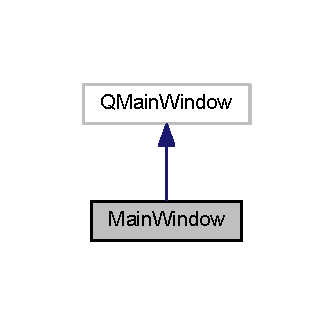
\includegraphics[width=160pt]{de/d4b/class_main_window__inherit__graph}
\end{center}
\end{figure}


Collaboration diagram for Main\+Window\+:\nopagebreak
\begin{figure}[H]
\begin{center}
\leavevmode
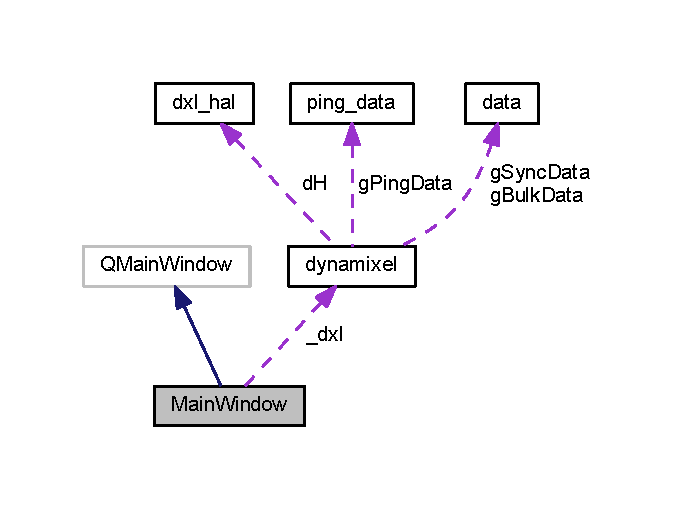
\includegraphics[width=324pt]{d0/db8/class_main_window__coll__graph}
\end{center}
\end{figure}
\subsection*{Public Member Functions}
\begin{DoxyCompactItemize}
\item 
\hyperlink{class_main_window_a8b244be8b7b7db1b08de2a2acb9409db}{Main\+Window} (Q\+Widget $\ast$parent=0)
\begin{DoxyCompactList}\small\item\em Default constructor. \end{DoxyCompactList}\item 
\hyperlink{class_main_window_ae98d00a93bc118200eeef9f9bba1dba7}{$\sim$\+Main\+Window} ()
\begin{DoxyCompactList}\small\item\em Default destructor. \end{DoxyCompactList}\end{DoxyCompactItemize}
\subsection*{Private Slots}
\begin{DoxyCompactItemize}
\item 
void \hyperlink{class_main_window_a1dd57ccb62bc6f5a361aba6e088dd2e1}{on\+\_\+action\+Options\+\_\+triggered} ()
\begin{DoxyCompactList}\small\item\em To select the options. \end{DoxyCompactList}\end{DoxyCompactItemize}
\subsection*{Private Attributes}
\begin{DoxyCompactItemize}
\item 
\hyperlink{classdynamixel}{dynamixel} \hyperlink{class_main_window_a07b4b97f6d4dfa77704b70d7dbbbebee}{\+\_\+dxl}
\begin{DoxyCompactList}\small\item\em Contains the comunication with the motors. \end{DoxyCompactList}\item 
Ui\+::\+Main\+Window $\ast$ \hyperlink{class_main_window_a35466a70ed47252a0191168126a352a5}{ui}
\begin{DoxyCompactList}\small\item\em Contains the user interface. \end{DoxyCompactList}\end{DoxyCompactItemize}


\subsection{Constructor \& Destructor Documentation}
\hypertarget{class_main_window_a8b244be8b7b7db1b08de2a2acb9409db}{}\index{Main\+Window@{Main\+Window}!Main\+Window@{Main\+Window}}
\index{Main\+Window@{Main\+Window}!Main\+Window@{Main\+Window}}
\subsubsection[{Main\+Window}]{\setlength{\rightskip}{0pt plus 5cm}Main\+Window\+::\+Main\+Window (
\begin{DoxyParamCaption}
\item[{Q\+Widget $\ast$}]{parent = {\ttfamily 0}}
\end{DoxyParamCaption}
)\hspace{0.3cm}{\ttfamily [explicit]}}\label{class_main_window_a8b244be8b7b7db1b08de2a2acb9409db}


Default constructor. 


\begin{DoxyCode}
4                                       :
5     QMainWindow(parent),
6     \hyperlink{class_main_window_a35466a70ed47252a0191168126a352a5}{ui}(\textcolor{keyword}{new} Ui::MainWindow)
7 \{
8     \hyperlink{class_main_window_a35466a70ed47252a0191168126a352a5}{ui}->setupUi(\textcolor{keyword}{this});
9     this->setWindowTitle(\textcolor{stringliteral}{"DeltaRobot Control"});
10     \hyperlink{class_main_window_a07b4b97f6d4dfa77704b70d7dbbbebee}{\_dxl}.\hyperlink{classdynamixel_a87960244d5846ae7583e37d2407eb61e}{initialize}(\textcolor{stringliteral}{"COM3"}, 1000000);
11 \}
\end{DoxyCode}
\hypertarget{class_main_window_ae98d00a93bc118200eeef9f9bba1dba7}{}\index{Main\+Window@{Main\+Window}!````~Main\+Window@{$\sim$\+Main\+Window}}
\index{````~Main\+Window@{$\sim$\+Main\+Window}!Main\+Window@{Main\+Window}}
\subsubsection[{$\sim$\+Main\+Window}]{\setlength{\rightskip}{0pt plus 5cm}Main\+Window\+::$\sim$\+Main\+Window (
\begin{DoxyParamCaption}
{}
\end{DoxyParamCaption}
)}\label{class_main_window_ae98d00a93bc118200eeef9f9bba1dba7}


Default destructor. 


\begin{DoxyCode}
14 \{
15     \textcolor{keyword}{delete} \hyperlink{class_main_window_a35466a70ed47252a0191168126a352a5}{ui};
16 \}
\end{DoxyCode}


\subsection{Member Function Documentation}
\hypertarget{class_main_window_a1dd57ccb62bc6f5a361aba6e088dd2e1}{}\index{Main\+Window@{Main\+Window}!on\+\_\+action\+Options\+\_\+triggered@{on\+\_\+action\+Options\+\_\+triggered}}
\index{on\+\_\+action\+Options\+\_\+triggered@{on\+\_\+action\+Options\+\_\+triggered}!Main\+Window@{Main\+Window}}
\subsubsection[{on\+\_\+action\+Options\+\_\+triggered}]{\setlength{\rightskip}{0pt plus 5cm}void Main\+Window\+::on\+\_\+action\+Options\+\_\+triggered (
\begin{DoxyParamCaption}
{}
\end{DoxyParamCaption}
)\hspace{0.3cm}{\ttfamily [private]}, {\ttfamily [slot]}}\label{class_main_window_a1dd57ccb62bc6f5a361aba6e088dd2e1}


To select the options. 


\begin{DoxyCode}
19 \{
20     \hyperlink{class_options_window}{OptionsWindow} o;
21     o.exec();
22     
23     \textcolor{keywordflow}{if} (o.result()) qDebug() << \textcolor{stringliteral}{"Acceptat"};
24     \textcolor{keywordflow}{else} qDebug() << \textcolor{stringliteral}{"Rebutjat"};
25 \}
\end{DoxyCode}


\subsection{Member Data Documentation}
\hypertarget{class_main_window_a07b4b97f6d4dfa77704b70d7dbbbebee}{}\index{Main\+Window@{Main\+Window}!\+\_\+dxl@{\+\_\+dxl}}
\index{\+\_\+dxl@{\+\_\+dxl}!Main\+Window@{Main\+Window}}
\subsubsection[{\+\_\+dxl}]{\setlength{\rightskip}{0pt plus 5cm}{\bf dynamixel} Main\+Window\+::\+\_\+dxl\hspace{0.3cm}{\ttfamily [private]}}\label{class_main_window_a07b4b97f6d4dfa77704b70d7dbbbebee}


Contains the comunication with the motors. 

\hypertarget{class_main_window_a35466a70ed47252a0191168126a352a5}{}\index{Main\+Window@{Main\+Window}!ui@{ui}}
\index{ui@{ui}!Main\+Window@{Main\+Window}}
\subsubsection[{ui}]{\setlength{\rightskip}{0pt plus 5cm}Ui\+::\+Main\+Window$\ast$ Main\+Window\+::ui\hspace{0.3cm}{\ttfamily [private]}}\label{class_main_window_a35466a70ed47252a0191168126a352a5}


Contains the user interface. 



The documentation for this class was generated from the following files\+:\begin{DoxyCompactItemize}
\item 
\hyperlink{mainwindow_8h}{mainwindow.\+h}\item 
\hyperlink{mainwindow_8cpp}{mainwindow.\+cpp}\end{DoxyCompactItemize}

\hypertarget{class_options_servos}{}\section{Options\+Servos Class Reference}
\label{class_options_servos}\index{Options\+Servos@{Options\+Servos}}


Inheritance diagram for Options\+Servos\+:
% FIG 0


Collaboration diagram for Options\+Servos\+:
% FIG 1
\subsection*{Public Member Functions}
\begin{DoxyCompactItemize}
\item 
\hypertarget{class_options_servos_a7bb41f5698acc37739be335f582003bc}{}{\bfseries Options\+Servos} (Q\+Widget $\ast$parent=0)\label{class_options_servos_a7bb41f5698acc37739be335f582003bc}

\end{DoxyCompactItemize}


The documentation for this class was generated from the following files\+:\begin{DoxyCompactItemize}
\item 
optionsservos.\+h\item 
optionsservos.\+cpp\end{DoxyCompactItemize}

\hypertarget{class_options_window}{}\section{Options\+Window Class Reference}
\label{class_options_window}\index{Options\+Window@{Options\+Window}}


{\ttfamily \#include $<$optionswindow.\+h$>$}



Inheritance diagram for Options\+Window\+:\nopagebreak
\begin{figure}[H]
\begin{center}
\leavevmode
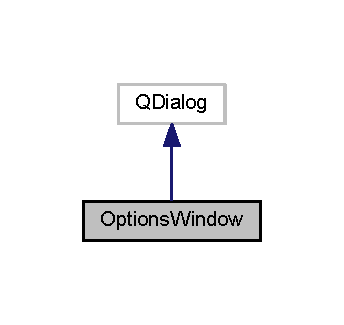
\includegraphics[width=165pt]{d3/d77/class_options_window__inherit__graph}
\end{center}
\end{figure}


Collaboration diagram for Options\+Window\+:\nopagebreak
\begin{figure}[H]
\begin{center}
\leavevmode
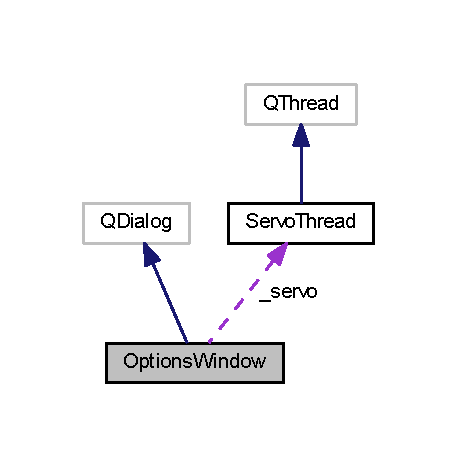
\includegraphics[width=165pt]{dd/d04/class_options_window__coll__graph}
\end{center}
\end{figure}
\subsection*{Public Member Functions}
\begin{DoxyCompactItemize}
\item 
\hyperlink{class_options_window_ac7ba16f211c07e2114015407c722840b}{Options\+Window} (Q\+Widget $\ast$parent=0)
\item 
\hyperlink{class_options_window_a034c885fe8bb4416e732a9571d14a6b4}{$\sim$\+Options\+Window} ()
\end{DoxyCompactItemize}
\subsection*{Private Slots}
\begin{DoxyCompactItemize}
\item 
void \hyperlink{class_options_window_aeb3e7dca619cd95e750e4575013be313}{on\+\_\+option\+\_\+current\+Item\+Changed} (Q\+List\+Widget\+Item $\ast$item, Q\+List\+Widget\+Item $\ast$)
\begin{DoxyCompactList}\small\item\em When the current selected item changes. \end{DoxyCompactList}\end{DoxyCompactItemize}
\subsection*{Private Attributes}
\begin{DoxyCompactItemize}
\item 
Ui\+::\+Options\+Window $\ast$ \hyperlink{class_options_window_a8347442d5b3b670e8fff0c4102db1f88}{ui}
\begin{DoxyCompactList}\small\item\em Containsh the G\+U\+I. \end{DoxyCompactList}\end{DoxyCompactItemize}


\subsection{Constructor \& Destructor Documentation}
\hypertarget{class_options_window_ac7ba16f211c07e2114015407c722840b}{}\index{Options\+Window@{Options\+Window}!Options\+Window@{Options\+Window}}
\index{Options\+Window@{Options\+Window}!Options\+Window@{Options\+Window}}
\subsubsection[{Options\+Window}]{\setlength{\rightskip}{0pt plus 5cm}Options\+Window\+::\+Options\+Window (
\begin{DoxyParamCaption}
\item[{Q\+Widget $\ast$}]{parent = {\ttfamily 0}}
\end{DoxyParamCaption}
)\hspace{0.3cm}{\ttfamily [explicit]}}\label{class_options_window_ac7ba16f211c07e2114015407c722840b}

\begin{DoxyCode}
4                                             :
5     QDialog(parent),
6     \hyperlink{class_options_window_a8347442d5b3b670e8fff0c4102db1f88}{ui}(\textcolor{keyword}{new} Ui::OptionsWindow)
7 \{
8     \hyperlink{class_options_window_a8347442d5b3b670e8fff0c4102db1f88}{ui}->setupUi(\textcolor{keyword}{this});
9     this->setWindowTitle(\textcolor{stringliteral}{"Options"});
10     
11     \hyperlink{class_options_window_a8347442d5b3b670e8fff0c4102db1f88}{ui}->stack->addWidget(\textcolor{keyword}{new} \hyperlink{class_options_servos}{OptionsServos});
12     \hyperlink{class_options_window_a8347442d5b3b670e8fff0c4102db1f88}{ui}->stack->addWidget(\textcolor{keyword}{new} QWidget);
13 \}
\end{DoxyCode}
\hypertarget{class_options_window_a034c885fe8bb4416e732a9571d14a6b4}{}\index{Options\+Window@{Options\+Window}!````~Options\+Window@{$\sim$\+Options\+Window}}
\index{````~Options\+Window@{$\sim$\+Options\+Window}!Options\+Window@{Options\+Window}}
\subsubsection[{$\sim$\+Options\+Window}]{\setlength{\rightskip}{0pt plus 5cm}Options\+Window\+::$\sim$\+Options\+Window (
\begin{DoxyParamCaption}
{}
\end{DoxyParamCaption}
)}\label{class_options_window_a034c885fe8bb4416e732a9571d14a6b4}

\begin{DoxyCode}
16 \{
17     \textcolor{keyword}{delete} \hyperlink{class_options_window_a8347442d5b3b670e8fff0c4102db1f88}{ui};
18 \}
\end{DoxyCode}


\subsection{Member Function Documentation}
\hypertarget{class_options_window_aeb3e7dca619cd95e750e4575013be313}{}\index{Options\+Window@{Options\+Window}!on\+\_\+option\+\_\+current\+Item\+Changed@{on\+\_\+option\+\_\+current\+Item\+Changed}}
\index{on\+\_\+option\+\_\+current\+Item\+Changed@{on\+\_\+option\+\_\+current\+Item\+Changed}!Options\+Window@{Options\+Window}}
\subsubsection[{on\+\_\+option\+\_\+current\+Item\+Changed}]{\setlength{\rightskip}{0pt plus 5cm}void Options\+Window\+::on\+\_\+option\+\_\+current\+Item\+Changed (
\begin{DoxyParamCaption}
\item[{Q\+List\+Widget\+Item $\ast$}]{item, }
\item[{Q\+List\+Widget\+Item $\ast$}]{}
\end{DoxyParamCaption}
)\hspace{0.3cm}{\ttfamily [private]}, {\ttfamily [slot]}}\label{class_options_window_aeb3e7dca619cd95e750e4575013be313}


When the current selected item changes. 


\begin{DoxyCode}
23 \{
24     \textcolor{keywordflow}{if} (item->text() == \textcolor{stringliteral}{"Servos"}) \{
25         qDebug() << \textcolor{stringliteral}{"Servos"};
26         \hyperlink{class_options_window_a8347442d5b3b670e8fff0c4102db1f88}{ui}->stack->setCurrentIndex(0);
27     \}
28     \textcolor{keywordflow}{else} \{
29         \hyperlink{class_options_window_a8347442d5b3b670e8fff0c4102db1f88}{ui}->stack->setCurrentIndex(1);
30     \}
31 \}
\end{DoxyCode}


\subsection{Member Data Documentation}
\hypertarget{class_options_window_a8347442d5b3b670e8fff0c4102db1f88}{}\index{Options\+Window@{Options\+Window}!ui@{ui}}
\index{ui@{ui}!Options\+Window@{Options\+Window}}
\subsubsection[{ui}]{\setlength{\rightskip}{0pt plus 5cm}Ui\+::\+Options\+Window$\ast$ Options\+Window\+::ui\hspace{0.3cm}{\ttfamily [private]}}\label{class_options_window_a8347442d5b3b670e8fff0c4102db1f88}


Containsh the G\+U\+I. 



The documentation for this class was generated from the following files\+:\begin{DoxyCompactItemize}
\item 
\hyperlink{optionswindow_8h}{optionswindow.\+h}\item 
\hyperlink{optionswindow_8cpp}{optionswindow.\+cpp}\end{DoxyCompactItemize}

\hypertarget{structping__data}{}\section{ping\+\_\+data Struct Reference}
\label{structping__data}\index{ping\+\_\+data@{ping\+\_\+data}}


{\ttfamily \#include $<$dynamixel.\+h$>$}

\subsection*{Public Attributes}
\begin{DoxyCompactItemize}
\item 
int \hyperlink{structping__data_afa48124c46271b97615e464bfb0b31bc}{i\+I\+D}
\item 
int \hyperlink{structping__data_a21475c3d8b2629e66cd2c1227c648489}{i\+Model\+No}
\item 
int \hyperlink{structping__data_a4a340fb47423b484b48237ceb5b39ef4}{i\+Firm\+Ver}
\end{DoxyCompactItemize}


\subsection{Member Data Documentation}
\hypertarget{structping__data_a4a340fb47423b484b48237ceb5b39ef4}{}\index{ping\+\_\+data@{ping\+\_\+data}!i\+Firm\+Ver@{i\+Firm\+Ver}}
\index{i\+Firm\+Ver@{i\+Firm\+Ver}!ping\+\_\+data@{ping\+\_\+data}}
\subsubsection[{i\+Firm\+Ver}]{\setlength{\rightskip}{0pt plus 5cm}int ping\+\_\+data\+::i\+Firm\+Ver}\label{structping__data_a4a340fb47423b484b48237ceb5b39ef4}
\hypertarget{structping__data_afa48124c46271b97615e464bfb0b31bc}{}\index{ping\+\_\+data@{ping\+\_\+data}!i\+I\+D@{i\+I\+D}}
\index{i\+I\+D@{i\+I\+D}!ping\+\_\+data@{ping\+\_\+data}}
\subsubsection[{i\+I\+D}]{\setlength{\rightskip}{0pt plus 5cm}int ping\+\_\+data\+::i\+I\+D}\label{structping__data_afa48124c46271b97615e464bfb0b31bc}
\hypertarget{structping__data_a21475c3d8b2629e66cd2c1227c648489}{}\index{ping\+\_\+data@{ping\+\_\+data}!i\+Model\+No@{i\+Model\+No}}
\index{i\+Model\+No@{i\+Model\+No}!ping\+\_\+data@{ping\+\_\+data}}
\subsubsection[{i\+Model\+No}]{\setlength{\rightskip}{0pt plus 5cm}int ping\+\_\+data\+::i\+Model\+No}\label{structping__data_a21475c3d8b2629e66cd2c1227c648489}


The documentation for this struct was generated from the following file\+:\begin{DoxyCompactItemize}
\item 
\hyperlink{dynamixel_8h}{dynamixel.\+h}\end{DoxyCompactItemize}

\hypertarget{class_x_joystick}{}\section{X\+Joystick Class Reference}
\label{class_x_joystick}\index{X\+Joystick@{X\+Joystick}}


The \hyperlink{class_x_joystick}{X\+Joystick}\textquotesingle{}s class is used to control the S\+F\+M\+L Joystick\textquotesingle{}s class with {\itshape signals and slots}  




{\ttfamily \#include $<$xjoystick.\+h$>$}



Inheritance diagram for X\+Joystick\+:
% FIG 0


Collaboration diagram for X\+Joystick\+:
% FIG 1
\subsection*{Classes}
\begin{DoxyCompactItemize}
\item 
struct \hyperlink{struct_x_joystick_1_1_info}{Info}
\begin{DoxyCompactList}\small\item\em Struct to handle the info. \end{DoxyCompactList}\end{DoxyCompactItemize}
\subsection*{Public Slots}
\begin{DoxyCompactItemize}
\item 
\hypertarget{class_x_joystick_a2052bd66345c8447a91902289ec6516f}{}void \hyperlink{class_x_joystick_a2052bd66345c8447a91902289ec6516f}{update} ()\label{class_x_joystick_a2052bd66345c8447a91902289ec6516f}

\begin{DoxyCompactList}\small\item\em Updates all data. \end{DoxyCompactList}\end{DoxyCompactItemize}
\subsection*{Signals}
\begin{DoxyCompactItemize}
\item 
\hypertarget{class_x_joystick_a46cf0117954ff155a3b55e9125e0b8d3}{}void \hyperlink{class_x_joystick_a46cf0117954ff155a3b55e9125e0b8d3}{changed} ()\label{class_x_joystick_a46cf0117954ff155a3b55e9125e0b8d3}

\begin{DoxyCompactList}\small\item\em Emmitted when a joystick is connected or disconnected. \end{DoxyCompactList}\end{DoxyCompactItemize}
\subsection*{Public Member Functions}
\begin{DoxyCompactItemize}
\item 
\hypertarget{class_x_joystick_a1d4f55adbffae86916947f248c9e5454}{}\hyperlink{class_x_joystick_a1d4f55adbffae86916947f248c9e5454}{X\+Joystick} (int I\+D=-\/1, float filter=0.\+001)\label{class_x_joystick_a1d4f55adbffae86916947f248c9e5454}

\begin{DoxyCompactList}\small\item\em Default constructor. \end{DoxyCompactList}\item 
\hypertarget{class_x_joystick_a14ebfadbb78639e533368c620f8cdcb8}{}\hyperlink{class_x_joystick_a14ebfadbb78639e533368c620f8cdcb8}{$\sim$\+X\+Joystick} ()\label{class_x_joystick_a14ebfadbb78639e533368c620f8cdcb8}

\begin{DoxyCompactList}\small\item\em Default destructor. \end{DoxyCompactList}\item 
\hypertarget{class_x_joystick_a1b65862348fb552e9607c37e1bd2a90d}{}int \hyperlink{class_x_joystick_a1b65862348fb552e9607c37e1bd2a90d}{amount} ()\label{class_x_joystick_a1b65862348fb552e9607c37e1bd2a90d}

\begin{DoxyCompactList}\small\item\em Amount of joysticks connected. \end{DoxyCompactList}\item 
\hypertarget{class_x_joystick_a8323d85b5923ee80e619e685267d9e18}{}bool \hyperlink{class_x_joystick_a8323d85b5923ee80e619e685267d9e18}{any\+Connected} ()\label{class_x_joystick_a8323d85b5923ee80e619e685267d9e18}

\begin{DoxyCompactList}\small\item\em True if there\textquotesingle{}s any joystick connected. \end{DoxyCompactList}\item 
\hypertarget{class_x_joystick_ab8e3e56c7b8f6f0dec911f351b4b361e}{}Q\+Vector$<$ \hyperlink{struct_x_joystick_1_1_info}{Info} $>$ \hyperlink{class_x_joystick_ab8e3e56c7b8f6f0dec911f351b4b361e}{available} ()\label{class_x_joystick_ab8e3e56c7b8f6f0dec911f351b4b361e}

\begin{DoxyCompactList}\small\item\em Returns the system available joysticks. \end{DoxyCompactList}\item 
\hypertarget{class_x_joystick_ad501613a09d6fc07a7054b8d6a8e83f1}{}bool \hyperlink{class_x_joystick_ad501613a09d6fc07a7054b8d6a8e83f1}{button} (int n)\label{class_x_joystick_ad501613a09d6fc07a7054b8d6a8e83f1}

\begin{DoxyCompactList}\small\item\em Returns the button state. \end{DoxyCompactList}\item 
\hypertarget{class_x_joystick_afb2d3fd919ba601fa8709bb97e1e0d48}{}int \hyperlink{class_x_joystick_afb2d3fd919ba601fa8709bb97e1e0d48}{button\+Count} ()\label{class_x_joystick_afb2d3fd919ba601fa8709bb97e1e0d48}

\begin{DoxyCompactList}\small\item\em Returns the number of buttons. \end{DoxyCompactList}\item 
int \hyperlink{class_x_joystick_a69ccd5ca34996e0e6b5b99ea7ddb4a5f}{current} ()
\item 
\hypertarget{class_x_joystick_ac72effd86a10e586deb6418db0b794fe}{}Q\+Vector$<$ P $>$ \hyperlink{class_x_joystick_ac72effd86a10e586deb6418db0b794fe}{get\+Axis} ()\label{class_x_joystick_ac72effd86a10e586deb6418db0b794fe}

\begin{DoxyCompactList}\small\item\em Returns all the Joystick\textquotesingle{}s axis and it\textquotesingle{}s names. \end{DoxyCompactList}\item 
\hypertarget{class_x_joystick_a436e8cb1940316d7ba3d0dd8d1f6002b}{}void \hyperlink{class_x_joystick_a436e8cb1940316d7ba3d0dd8d1f6002b}{axis\+Press} (unsigned char a, float value=100)\label{class_x_joystick_a436e8cb1940316d7ba3d0dd8d1f6002b}

\begin{DoxyCompactList}\small\item\em To mantain an axis in a certain value. \end{DoxyCompactList}\item 
\hypertarget{class_x_joystick_a55531560621ea0aedf9cf7f123294c79}{}void \hyperlink{class_x_joystick_a55531560621ea0aedf9cf7f123294c79}{axis\+Release} (unsigned char a)\label{class_x_joystick_a55531560621ea0aedf9cf7f123294c79}

\begin{DoxyCompactList}\small\item\em To release an axis and restore it\textquotesingle{}s value with the joystick. \end{DoxyCompactList}\item 
\hypertarget{class_x_joystick_afc3d48cab266b9596182229eb0df4384}{}const float \& \hyperlink{class_x_joystick_afc3d48cab266b9596182229eb0df4384}{operator\mbox{[}$\,$\mbox{]}} (int n) const \label{class_x_joystick_afc3d48cab266b9596182229eb0df4384}

\begin{DoxyCompactList}\small\item\em Returns the \textquotesingle{}n\textquotesingle{} axis value. \end{DoxyCompactList}\item 
\hypertarget{class_x_joystick_abfc58c4863c6ae9a4b4b1169114903e0}{}bool \hyperlink{class_x_joystick_abfc58c4863c6ae9a4b4b1169114903e0}{select} (int s)\label{class_x_joystick_abfc58c4863c6ae9a4b4b1169114903e0}

\begin{DoxyCompactList}\small\item\em Selects the especified joystick. \end{DoxyCompactList}\end{DoxyCompactItemize}


\subsection{Detailed Description}
The \hyperlink{class_x_joystick}{X\+Joystick}\textquotesingle{}s class is used to control the S\+F\+M\+L Joystick\textquotesingle{}s class with {\itshape signals and slots} 

\subsection{Member Function Documentation}
\hypertarget{class_x_joystick_a69ccd5ca34996e0e6b5b99ea7ddb4a5f}{}\index{X\+Joystick@{X\+Joystick}!current@{current}}
\index{current@{current}!X\+Joystick@{X\+Joystick}}
\subsubsection[{current}]{\setlength{\rightskip}{0pt plus 5cm}int X\+Joystick\+::current (
\begin{DoxyParamCaption}
{}
\end{DoxyParamCaption}
)\hspace{0.3cm}{\ttfamily [inline]}}\label{class_x_joystick_a69ccd5ca34996e0e6b5b99ea7ddb4a5f}
Returns the current selected joystick, -\/1 if there\textquotesingle{}s no selected joystick 

The documentation for this class was generated from the following files\+:\begin{DoxyCompactItemize}
\item 
xjoystick.\+h\item 
xjoystick.\+cpp\end{DoxyCompactItemize}

%--- End generated contents ---

% Index
\backmatter
\newpage
\phantomsection
\clearemptydoublepage
\addcontentsline{toc}{chapter}{Index}
\printindex

\end{document}
